%-------------------------------------------------------------------------------
\vspace{-5mm}
\begin{abstract}
We test whether the availability of the emergency contraceptive (``morning 
after'') pill in the absence of legalised abortion can have effects similar to 
those of other large-scale contraceptive reforms. To do so we examine a 
quasi-experimental policy reform occurring in Chile in 2008. Using vital 
statistics covering all births and fetal deaths over the period 2006-2012, we 
show that the availability of the morning after pill reduces pregnancy and early 
gestation fetal death, which we argue proxy for illegal abortions. These effects 
are particularly pronounced among teenagers and young women: point estimates 
suggest a 6.9\% reduction in teenage pregnancy and 4.2\% reduction for 20-34 
year olds. We suggest that diffusion of the morning after pill between treatment 
and control areas played an important role, and suggest a way to estimate 
unbiased treatment effects of the reform in the presence of local spillovers. 
Our results suggest that in the context of Chile, a country with among the most 
conservative abortion laws in the world, the emergency contraceptive pill may 
have effects nearly as large as various abortion reforms observed in other 
contexts.
\\ \JELs 
\end{abstract}

\section{Introduction}
Undesired pregnancy---particularly among young and adolescent women---is a
considerable contributor to poor maternal and child outcomes, and to a lack of
intergenerational mobility.  The last half-century has seen a remarkable 
increase in contraceptive technology, with considerable impacts on rates of such
undesired pregnancy and with far-reaching consequences for the social and 
productive structure of modern society. The widespread introduction of the oral 
contraceptive pill has brought with it lower birth rates, delays in childbearing 
and marriage, higher rates of human capital attainment and labour market 
participation for women \citep{AngristEvans1996,Bailey2006,GoldinKatz2002a,
GoldinKatz2002b}, reductions in the gender wage differential 
\citep{Baileyetal2012}, and, theoretically at least, more empowered women 
\citep{ChiapporiOreffice2008}.  In the long-run, these outcomes have led to 
generations of children less likely to have divorced parents, and more likely to 
live with college educated mothers \citep{OltmansHungerman2012}.

While the contraceptive pill has had a remarkable impact on a woman's capability
to control the timing of her fertility decisions, these treatments require an
expensive ongoing investment, which is difficult or impractical for certain 
groups of women.  In contrast to the rich literature on the effects of the 
contraceptive pill, very little evidence is available regarding the effects of 
post-coital (non-abortive) birth control.  In this paper \person examine the 
effect of fully-subsidised provision of the emergency contraceptive (EC) pill.  
This so called ``morning after pill'' offers an alternative form of 
contraception in cases where other forms were not used or failed during 
intercourse, or in the case of rape.

The scarce existing literature on this topic suggests that the EC pill may have 
had surprisingly little effect on both pregnancy and abortion 
\citep{Grossetal2014,Durrance2013}. Compared to the large body of evidence 
suggesting that contraceptive technologies such as the oral contraceptive and 
legal abortion can have significant and important effects on pregnancy rates, 
empirical studies of the effect of the EC pill have found small or non-existent 
shifts in fertility outcomes despite high rates of use\footnote{For example, 
the CDC reports that in the United States between 2006 and 2010, 11\% (5.8 
million) women aged between 15 and 44 used the emergency contraceptive pill at 
least once.  Among 20-24 year olds, the rate is even higher, at 23\% 
\citep{Danielsetal2013}.}.  However, existing analyses of the effect of the 
morning after pill on birth rates have been limited in terms of the contexts 
examined.  Existing quasi-experimental studies in the literature are focused on 
the United States, where abortion is legal, and hence the scope of the EC on 
net birth rates is likely to be limited, especially if abortion and the EC pill
act as substitutable technologies.\footnote{Indeed, this is explicitly 
suggested, although untested, in the economic literature. \citet{Grossetal2014}, 
in one of the few quasi-experimental studies of the EC pill, write a model of 
contraceptive use where use of the EC pill depends on the outside cost of 
abortion. They find small effects in the USA, however state:
     \begin{quote}
     ``This paper studies the effect of EC during a time period in which
     abortion was legal. The effect of EC might be very different [were]
     abortion to be illegal (Bailey, Guldi, \& Hershbein, 2013; Joyce,
     2013).
     \end{quote}}

However, in many countries and regions, abortion is highly regulated, allowed
in only extreme cases, or even outlawed entirely.  Recent figures suggest that 
only one third of the world's governments currently allow elective abortion or 
abortion for economic or social reasons, with this number being considerably 
lower in developing regions with high rates of fertility \citep{UN2014}.  For 
areas in which abortion is not decriminalised, it is of considerable interest 
to determine whether the arrival of the EC pill in the isolation of abortion 
is sufficient to provide similarly remarkable changes in fertility rates as 
those observed with the historical arrival of the first wave of contraceptive 
technologies to other areas.

%In the case of Chile, prior to the 
%availability of the EC pill, abortion was illegal in all circumstances, and 
%clandestine abortions resulting in hospitalisation resulted in incarceration in 
%some cases.\footnote{Chile is one of only seven countries in which abortion is 
%criminalized in all circumstances, including the cases of fetal inviability, 
%risk to the life of the mother, and rape.  [CITE] and numbers.}

A considerable literature on the effect of both the oral contraceptive pill
and abortion, in USA and in other countries, suggests that both may have direct
effects on rates of teen births of around $-4$ to $-9$\%.  Table
\ref{TEENtab:lit} provides a summary of the range of estimated effects found in
economic studies of contraceptive reforms.  Although not a comprehensive meta-%
analysis, these quasi-experimental studies examining different contexts and
national reforms often find broadly similar effects, suggesting that both
abortion and the oral contraceptive pill alone resulted in significant 
reductions in births. In USA, these estimates suggest that both methods reduce 
childbearing at a young age by about 5.5\% (mean estimate), while in Romania 
and Nepal, the effects are closer to 7\%.  In this paper, we examine whether the 
morning after pill alone (where legal abortion is not available) could have 
effects of similar magnitude and importance.

In order to examine the effect that the EC pill can have on mothers and children 
when abortion is \emph{not} available, we turn to a particular empirical example.  
We focus on a plausibly exogenous policy decision in Chile which affects a 
woman's access to the fully subsidised emergency contraceptive pill.  We find 
considerable evidence that, at least in the case of Chile, (a country with no 
access to legal abortion in any circumstances\footnote{In Chile abortion is 
illegal in all circumstances, and clandestine abortions resulting in 
hospitalisation result in incarceration in some cases \citep{ShepardCasas2007}.  
Chile is one of only six countries in which abortion is criminalized in all 
circumstances, including the cases of fetal inviability, risk to the life of the 
mother, and rape \citep{UN2014}.}), access to emergency contraception does have 
significant effects on births, and that these effects are concentrated on 
teenagers and young women.  We also find suggestive evidence that morning after 
pill availability results in a reduction of women having to recur to illegal and 
risky clandestine abortions.  With the arrival of the morning after pill, we 
observe a reduction in early term fetal deaths in reform areas, and no similar 
reduction in non-reform areas, while no similar effect is observed for late term 
fetal deaths.  In the case of both births and deaths, the observed effects appear 
to be transversal rather than being centred on more highly educated or 
high-income women. 

The reform under examination comes from a series of constitutional challenges 
between 2005-2008, which meant that the introduction of the emergency contraceptive 
pill in Chile was entirely controlled by the Supreme Court and Constitutional 
Tribunals.  Legal challenges resulted in the 2008 finding that it would be illegal 
for all nationally run health centres and hospitals to prescribe the emergency 
contraceptive pill, however that in each of the 346 municipalities of Chile health 
centres were at liberty to do so.  This resulted  in a situation in which a woman's 
access to the pill entirely depended upon the decisions taken by her mayor.  Due 
to this reform it is shown that around half the municipalities in Chile made the 
pill available, while the other half did not.  Using administrative birth data and 
censal population data, we observe each woman's pregnancy status in each year and 
the outcome of each of these pregnancies, as well as municipal-level pregnancy and 
fetal death rates.

Using this reform, we estimate the effect that the staggered arrival of the 
emergency contraceptive had on women and children, including its effect on births 
and fetal deaths. The arrival of this new technology is associated with significant 
reductions in these outcomes.  Further, the effects identified are of considerable
magnitude.  It is estimated that among teenage girls, the widespread availability 
of emergency contraception reduces births by around 7\%, and reduces rates of early
term fetal death (which we argue may reflect illegal abortion) by approximately 30\%. 
Among older women, the reductions in births and early term fetal deaths are more 
moderate, however still quantitatively important.  For example, among 20-34 year 
olds, the emergency contraceptive pill reduces births by an estimated 4.2\% and 
appears to reduce illegal abortion by around 9\%.

\nocite{Goldin2006, Bailey2011}
\nocite{KearnerLevine2009}
\nocite{Ananatetal2007,ThomasDouglas1996,Levineetal1996}

Naive estimates of the effect of the morning after pill on pregnancies, abortions, 
and other outcomes, are based on the assumption that the arrival of the emergency 
contraceptive to approximately half of the women in the country had no effect on 
those women who did not live in areas where the EC pill was available.  We examine 
the validity of this assumption by comparing women who live `close' to areas where 
the EC pill was available to those who live considerably further away.  It is shown 
that significant treatment spillovers may occur, and so suggested that naive 
estimates of the effect of the emergency contraceptive pill may significantly 
underestimate the true effect of the expansion of availability in Chile.

Given the spatial nature of these spillovers, a methodology is proposed which
allows for the recovery of a consistent treatment effect even in the presence
of local spillovers.  It is shown that under certain assumptions regarding the
nature of the stable unit treatment value assumption, the estimated treatment 
effect will be significantly attenuated if this consideration is not made.
We then propose a number of ways to determine which control clusters should
be considered `close to' treatment clusters.  It is shown that for the morning
after pill, treatment spillover is a quantitatively important consideration,
and that in some groups, diffusion may exist for anywhere up to 25km from a
treatment location.

This study makes a number of contributions.  Foremost, it is one of the first%
---if not the first---study of the effects of emergency contraception using 
complete microdata on births and deaths at a national scale. It is also the first 
large scale study of which the authors are aware which addresses these questions 
in a country other than the United States.  This is of considerable importance 
given that Chile, the country under study here, does not offer legal abortion, 
and so the emergency contraceptive pill is the first legal mechanism for 
post-coital fertility control.  The context studied here offers lessons on the 
nature of contraceptive reforms, and whether emergency contraceptives in a 
context of high rates of undesired pregnancy and few outside options are 
sufficient to have effects over observed birth rates.
%\footnote{This is not to suggest that \emph{no} post-coital
%contraceptive options exist.  Given the lack of a legal solution, Misoprostol
%accessed on the black market is overwhelmingly to most common method used to
%interrupt undesired pregancies (Casas 2014).}

The results of this study add to the nascent literature on the emergency 
contraceptive pill.  Recent studies such as \citet{Grossetal2014} and 
\citet{Durrance2013} which have been the first to address this question in 
the economic literature have provided evidence to suggest that the effects of 
this technology may be minor.  Here we offer considerable evidence to the 
contrary, suggesting that the expansion in the availability of emergency 
contraceptives may offer important effects in certain countries, with large 
impacts on pregnancy and abortion rates, especially among young women.

Finally, \person raise a number of points regarding the estimation of 
treatment effects in the presence of spillovers between treatment and control
clusters.  This is fundamentally different to, despite sharing some 
characteristics with, the literature on estimating treatment effects in the 
presence of spillovers between treated and non-treated individuals within 
treatment clusters.  \Person suggest that even in the presence of such 
spillovers, unbiased treatment effects can be estimated if these spillovers
occur in a predictable way, as is likely to be the case when distance to 
treatment varies in an exogenous manner. \Person propose a number of flexible
ways to consider estimating treatment effects in these circumstances.

%%In what remains of this paper \person first provide background regarding the
%%emergency contraceptive pill, and the reform under study in Chile in section
%%\ref{TEENscn:background}.  Section \ref{TEENscn:Data} discusses the 
%%administrative datasets we will use to assess the effects of the reform, while 
%%\ref{TEENscn:ID} discusses identification and methodology.  In section 
%%\ref{TEENscn:results} \person present results on the contraceptive's effect on 
%%births, abortions and aggregate human capital endowments.  Finally, section 
%%\ref{TEENscn:conclusion} concludes.
  
% > GENERALISE REFORM PART TO DISCUSS FERTILITY IN CHILE
% YUZPE: DIDES 2010 ASK, ONLY 3 OF THE COMUNAS ALLUDE TO ITS USE.
%% IN OFFICIAL DOCUMENTS RELEASED BY THE GOVERNMENT, INCLUDING THEIR GUIDE TO
%% TEEN PREGNANCY, THERE IS NO MENTION OF THIS METHOD.  IN THE PREVAILING LAWS
%% IN BOTH 2006 AND 2012, THERE IS ALSO NO MENTIONS OF THIS METHOD. 
%*******************************************************************************
\section{The History of the Emergency Contraceptive Pill}
\label{TEENscn:background}
\subsection{The Emergency Contraceptive Pill}
The emergency contraceptive pill is a hormonal treatment which can be used 
within 5 days of an unprotected sexual relationship to reduce the probability
of conception.  There are a number of alternative types of emergency 
contraceptive pills, however principally these are composed of doses of the 
progestin levonogestrel, or a combined dose of estrogen and progestin. 
Typically these are taken as a single pill or two pills in a 12 hour period
\citep{vonHertzenetal2002}, however similar doses of hormones can be obtained 
by combining normal birth control pills \citep{Ellersonetal1998}.  

This form of contraception has been shown to be relatively effective at 
avoiding undesired pregnancy.  Estimates of around 75\%-85\% effectiveness 
based on typical usage are common, depending upon the method of emergency 
contraception used.\footnote{The WHO's \citet{WHO1998}, for example suggests 
that a levonogestrel routine reduces pregnancy rates by 85\%, with a 95\% 
confidence interval of 74-93\%.}  The success of these treatments is dependent
upon the delay between intercourse and taking the drug, so widespread---or at 
least quickly available---access is important in reducing undesired pregnancies.
While most effective when taken within 12 hours after intercourse, 
effectiveness can continue when taken within as much as 120 hours
\citep{vonHertzenetal2002}.

The emergency contraceptive pill is not an abortive agent, but rather is a 
`postcoital contraceptive' which acts to prevent ovulation 
\citep{Novikovaetal2007, Noeetal2011}. This contraceptive method has been of 
clinical interest since at least the late 1960s \citep{Demers1971}, however 
access to these methods, either by prescription or over the counter, is still 
not universal.  The fact that emergency contraception is non-abortive has 
meant that it is available in many countries in which abortion is absolutely 
prohibited, or prohibited in all cases except where concerns for maternal 
survival exist.  Some countries have made the EC pill available as early as 
the mid-1980s \citep{UKFPA2006}, while many more countries have legalised 
the EC pill during the last decade.

\subsection{The History of EC Pill in Chile}
\label{TEENsscn:Chile}
The introduction of the emergency contraceptive pill in Chile has followed 
a complicated path, with early legislation frequently blocked by conservative 
groups in office and in civil society.\footnote{The Chilean political 
framework is marked by a strong conservative axis, and a constitution which 
favours the maintenance of the status quo in economic and social policies.  
This has been the case since the return to democracy in 1990, with an 
alliance of right wing parties (and some members of the presiding left wing 
coalition) who have ``resisted more liberal changes in the poorly named value 
judgements''  (\citet{CasasBecerra2008}, p.6, author's translation.)}  While 
initial discussions and administrative inquiries took place in 2001, it was 
not until 2005 that significant advances in legislature were made. In 
December of this year the Chilean Supreme Court determined that the Institute 
of Public Health---the pharmaceutical regularity body of Chile---was 
\emph{not} acting unconstitutionally by approving the provision of an 
emergency contraceptive drug on the pharmaceutical register.  However, this 
finding was quickly challenged by detractors, with cases presented before 
ordinary and Constitutional Tribunals \citep{CasasBecerra2008}.

These tribunals were followed by a number of years' worth of legislations and
litigations, which resulted in sporadic availability of the morning
after pill, occasionaly freely available from state clinics or by purchase in
private pharmacies.  However, these were generally short-lived and emergency
contraception was not consistently stocked, with both political and economic 
ramifications for groups providing access to the pill.\footnote{For example,
the subsecretary of health was removed from cabinet due to his announcement
in 2005 that emergency contraception would be available to all women who sought
it.}  Details regarding this intervening process and laws passed by parliament
theoretically requiring the provision of emergency contraception are discussed 
more fully in the online appendix to this paper.

The period of interest for this study follows a decision taken by the Chilean
Constitional Tribunal in 2008.  This finding, responding to a demand placed by
36 parlamentary deputies in 2006, made it expressly illegal for the centralised
health system to distribute the emergency contraceptive.  This requirement held
for all centres under direct administration of the national Ministry of Health,
but, fundamentally, provided all municipal-level centres and hospitals the 
freedom to distribute the pill.  Given that these centres are administered by 
the mayor of each municipality (or \emph{comuna}), the availability in each 
municipality was entirely under the control of the mayor \citep{Didesetal2011,
Didesetal2010,Didesetal2009}.\footnote{Of the 346 municipalities in Chile, 320
have their own health systems, while the remaining 26 depend entirely upon the
Ministry of Health.  These 320 municipalities make up 94\% of the population 
of Chile.  Municipal health centres make up the majority of health centres in 
Chile.  Of the 2501 registered health centres and hospitals, 2049 are under the
control of municipalities \citep{DEIS2013}.}  This resulted in a situation in
which around half of the municipalities in Chile distributed the morning after
pill freely, while the remaining half refused to distribute it, or to 
distribute it only in a very restrictive set of circumstances.  At the level
of the woman, her municipality's treatment status was essentially exogenously
determined, being based on the whim of the mayor or representative public 
health bodies in her area of residence.  We provide further discussion of the
mayor and municipality characteristics and EC provision in section 
\ref{TEENscn:ID}.  This idiosyncratic policy environment endured for 
approximately four years, until a law was passed mandating that the emergency 
contraceptive pill must be available to all women who request it.  This new 
law became operational in May of 2013.

The Chilean context is one in which emergency contraception may be expected to
have particularly important effects on pregnancy and maternal health.  Abortion
is entirely illegal in Chile, meaning that in the absence of emergency 
contraception, undesired or accidental pregnancies must either be taken to 
term, or a woman must risk undertaking a dangerous and illegal clandestine
abortion \citep{ShepardCasas2007}.  Figures on the frequency and method of 
clandestine abortion are unclear, however \citet{ShepardCasas2007} suggest that
the primary method is by taking the abortive drug misoprostol, which can be
legally prescribed for treatment of ulcers.  However, the cost of accessing 
this drug without prescription is high.  Dated (2007) figures suggest prices
of 38,000-50,000 Chilean pesos, or around one third of the minimum monthly wage
at this time.  Further discussion related to the contraceptive environment in 
Chile preceding and posterior to the reform are available in online appendix B.  

%--------------------------------------------------------------------------------
\section{Data}
\label{TEENscn:Data}
Population data from Chile comes from two main sources. The first is vital 
statistics data, recording births and fetal deaths which are provided by the 
Ministry of Health of the Government of Chile (MINSAL). This data provides 
microdata records covering greater than 99\% of all births and fetal deaths 
reported in aggregate data \citep{Bharadwajetal2013} in the country. Each entry 
records the occurrence of a birth or fetal death, characteristics of the mother 
(and if present the father) including her age, education, and muncipality of 
residence, as well as a number of charactersitics of the birth (including 
birthweight, gender, gestation and birth order) or the fetal death (weeks of 
gestation, birth order, cause of death). These data have been collected and 
reported in Chile since 1982, and, at the time of writing, are publicly 
available up to the year 2012. These vital statistics data for birth and
fetal deaths thus provide data on all pregnant women in the country who either 
give live birth, have a birth leading to fetal death or who miscarry in any 
hospital in the country.

Data on all women of reproductive age comes from the National Institute of 
Statistics of Chile (INE). The INE provides estimations of the number of women 
of each age living in each municipality in each year. These estimates are based 
on the decennial census, as well as net migration each year, and vital 
statistics on all births and deaths occurring to residents in the municipality 
(Instituto Nacional de Estadsticas, 2014). These two sources of data provide 
information on the number of women of fertile age living in each municipality, 
and the number of women pregnant in each municipality during the time period of 
interest. They can be merged at the level of the municipality, resulting in
counts of total number of births and non-pregnant women, and also the calculation 
of municipal-level rates of pregnancy (births/total women), and fetal deaths 
(deaths/total births).  We provide additional details regarding the vital 
statistics and population data and their structure and matching in the online
appendices provided with this paper.

This results in a total sample of 1,605,300 births and 13,063 fetal deaths
ocurring between 2006 and 2012 (inclusive).  The number of births per year in 
Chile has remained relatively stable over the last decade.  
Figure \ref{TEENfig:BirthDeath} displays total births, along with total fetal 
deaths during the period under study.  Total births vary between around 
220,000-250,000 per year, while total fetal deaths recorded in the Ministry of 
Health data (all fetal deaths in any hospitals or clinics in Chile), vary between 
1700 and 2100.



%%%The data of interest for this study comes from matched administrative data files 
%%%recording all live births and fetal deaths in Chile.  \Person use birth outcomes 
%%%for all women aged between 15 and 49 (inclusive) at some point during 2006-2011.  
%%%This is crossed with data recording all women in Chile and their municipality of
%%%residence, resulting in a record of each woman, and her pregnancy status in each 
%%%period (live birth, fetal death or no pregnancy).  Along with a woman's birth 
%%%status, we observe her baby's birth weight and gestational length in the case 
%%%that a birth or fetal death was recorded.\footnote{Since 1999, each baby born in 
%%%Chile (in public and private hospitals and in private homes with midwives) is 
%%%weighed and measured, and their gestational time is recorded.  This data is 
%%%collated by the Ministry of Health, and is available as a public birth weight 
%%%census.  As well as the baby's characteristics, the mother's education, age, 
%%%labour market status and municipality of residence is collected.  Similar 
%%%details are collected in the case that a woman enters hospital and suffers a 
%%%miscarriage.}

Our measure for the pill is a binary variable which records whether the 
emergency contraceptive was freely available to a woman upon request at her 
municipal health centre in the year before her birth outcome is observed.  We
consult two sources to collect data on pill availability.  First, in each of 
2009, 2010 and 2011 an independent survey was conducted, asking health care 
workers from each municipality whether they were able to prescribe the morning
after pill \citep{Didesetal2009,Didesetal2010,Didesetal2011}. This should 
directly reflect the decision by each mayor regarding whether his or her
municipality could prescribe the pill after the 2008 Constitutional ruling.  
In each case, survey respondents were also asked to list the circumstances in 
which they could prescribe the pill.  All municipalities which reported that
they could prescribe the pill freely to women were recorded as treated, while 
all others were recorded as untreated.\footnote{A small number of 
municipalities reported that they could prescribe the emergency contraceptive, 
however that this was only following cases of rape.  These municipalities were 
classed as \emph{un}treated given the lack of widespread availability.}  
Secondly, the Ministry of Health has made available administrative data on 
all pill requests and dispursements at municipality clinics and hospitals.  This
allows us to determine the veracity of the survey data discussed above, 
while also providing concrete numbers regarding the use of the emergency 
contraceptive pill following the reform of interest.  However, \person do not
use pill disbursements as the main measure of treatment.  \Person focus on
reported availability, given that disbursements are endogenous, and jointly
determined by demand as well as supply.\footnote{However, when we define EC
pill municipalities based on disbursements rather than reported willingness 
to prescribe, we find effect sizes which are largely similar.  These results
are presented as an online appendix.}

In total, 224 of Chile's 346 municipalities report being able to prescribe the 
pill in at least one year after the 2008 Tribunal result (see table 
\ref{TEENtab:SumStats}). Figure \ref{TEENfig:Pilltime} displays the quantity
of municipalities reporting pill disbursements over time.  Here, the number
of prescribers increases over time in line with greater awareness of the legality 
of distributing the emergency contraceptive pill.  While less than half of all
municipalities report pill availability in 2009, this has increased to around
two thirds by 2011.  Official records of pill prescriptions suggest reasonably
large fluctuations over time.  While nearly 8000 women were reported as 
requesting the pill in 2009, this fell to slightly under 4000 the following
year.  Recent figures suggest that this number has been stable at around 6000-%
7000 requests in 2011-2013 (the most recent two years have been omitted from
this study, and from graphical output, given that official birth records for
2013 are not yet finalised).  Figure \ref{TEENfig:PillGeo} displays
the geographic variation of pill availabilitly.  This suggests that the pill
is available in all parts of the country. With the exception of the large and 
very sparsely populated southern region of the country (the 
10\textsuperscript{th} region) which has no municipal health centres, no 
obvious spatial patterns exist.

\Person examine fetal deaths as a manner to proxy illegal abortion.  While it 
is certainly not the case that all (or even the majority) of fetal deaths 
observed in administrative data are results of abortive drugs, there is some
evidence that these are the result of abortion in some cases, although they are 
recorded in a number of different ways in official figures to avoid criminal 
charges against women \citep{ShepardCasas2007}.  To avoid concerns that 
reductions in fetal deaths may be simply due to greater investments in public
health, \person examine a number of subgroups of interest.  Firstly \person focus 
on deaths occurring between 1-20 weeks of gestation, as this is the period in 
which nearly all abortions are conducted.  Secondly, \person remove deaths which,
based on their ICD code,\footnote{The ICD refers to the International 
Classification of Disease, and refers to a set of standardised codes by which
deaths can be classed.  All deaths on the birth register report this code,
(the ICD-10).} are clearly not related to abortion, such as those due to 
congenital malformations, deformations and chromosomal abnormalities.  By
using this methodology, a clear validity check exists by comparing reductions
in fetal deaths during 1-20 weeks (which may represent abortions and should
respond to the morning after pill), to those occurring from week 21 and above,
which should be largely or entirely unaffected by emergency contraceptive
availability.

Full summary statistics are provided in Table \ref{TEENtab:SumStats}.  These
statistics are subdivided by whether or not the municipality has the pill in
a given year.  We see that there are some differences between pill and non-pill
municipalities, such as higher education and health spending in pill 
municipalities.  However, this is largely due to the fact that all years in which
the pill was observed occur after 2008 while non-pill status is observed over
the entire time period under study.  In order to test this more formally, in
table \ref{TEENtab:pillchoice} each municipality's EC pill status is regressed
on all observed municipality characteristics, mayor characteristics, as well as 
year and region fixed effects.  Unlike the raw summary statistics, this table 
suggests that those municipalities where the EC pill was prescribed do not look
remarkably different to areas where the EC was not prescribed, with two 
exceptions.  Of the observed time varying controls, differences (at a 5\% level)
are observed along the conservativeness of the mayor's party (which is negatively 
related to EC pill status), and by the degree to which condoms are also used in 
the region (which is positively related to EC pill availability).  As we discuss 
later in the paper, we address concerns that municipalities which do and do not 
prescribe the EC pill may differ in a way which threatens identification in a 
number of ways.  Firstly, we estimate full event studies to examine the 
plausibility of parallel trends, secondly, we weight using inverse-propensity 
scores, and thirdly, we include these time-varying controls in our regressions.

Longer time-series trends of the number of pregnancies in Chile are presented
in figures \ref{TEENfig:Trend1519} (births to 15-19 year old mothers) and 
\ref{TEENfig:Trend2034} (for 20-34 year olds).  These figures display the counts 
of total numbers of pregnancies, split by whether or not the municipality 
reported giving the EC pill in 2010.  While there are year-by-year fluctuations, 
from 2004 onwards, there is an increasing trend in the absolute number of 
pregnancies in both age groups.  This tendency reverts following the availability 
of the EC pill in municipal health centres.  While this reversion is seen in the 
whole country, it is extremely sharp in municipalities which report that the 
morning after pill was available when requested by women.  In the following 
sections, we examine this effect econometrically.

%********************************************************************************
\section{Methodology}
\label{TEENscn:ID}
\subsection{Flexible Differences-in-Differences Estimates}
\Person take advantage of the quasi-experimental nature of the expansion of the 
availability of the morning after pill to women in Chile.  A woman $i$, living
in municipality $j$ in year $t$ is considered as treated if public health 
centres report that the pill is available upon request.  A woman's child 
bearing status $birth_{ijt}$ is regressed on the availability of the pill 
($pill_{jt}$) in the preceding year:
\begin{equation}
 \label{TEENeqn:pill}
birth_{ijt} = \alpha + \delta\cdot \mathbb{I}\{Pill_{jt-1}\} + \phi_t + \eta_j + 
\eta_j\cdot t + X_{jt-1}\gamma + \varepsilon_{ijt}.
\end{equation}
In (\ref{TEENeqn:pill}), full municipality and year fixed effects are included,
and municipality-specific time trends are allowed.  Standard errors are 
estimated which allow for auto-correlation by municipality.  The identifying 
variation in availability of the pill is by municipality and year.  Prior to 
the legal reform the pill was unavailable to all women, while posterior to the
reform the pill was available to those women living in municipalities where the
mayor did not restrict access.\footnote{Prescribing the pill in a given year
after the reform does not imply that municipalities necessarily prescribe the 
pill in the years following.  For example, in some cases municipalities 
switched from 0 (pre-reform), to 1 (during reform), back to 0 (during reform), 
and then to 1 definitively (post-reform) after the EC pill was made legal in the 
whole country in 2013.
Our identification strategy takes advantage of this switching, given that 
$Pill_{jt}$ varies by municipality and time.}  This provides a flexible 
difference-in-differences (hereafter diff-in-diff) framework, and allows us to 
causally estimate the effect of the morning after pill if we believe that 
typical diff-in-diff assumptions hold.  Namely, we require that unobserved 
components $\varepsilon_{ijt}$ in the above specification evolve similarly over 
time in the treated and untreated municipalities.

Given the geographically disperse, and, as discussed in previous sections,
plausibly exogenous nature of the arrival of the morning after pill, we may be
willing to accept that this assumption is valid.  However, to minimise the 
potential that spurrious events confound the arrival of the pill, we 
progressively include higher order time trends and other factors that vary 
non-linearly over time across municipalities.  These factors, $X_{jt-1}$, 
include controls for political and social outcomes such as the mayor's party
(and implicitly the conservativeness of views), the degree of voter support for
the mayor, the mayor's gender, health and education inputs including staffing
and training investments, and time varying measures of female empowerment by
municipality.

In our principal specification, we estimate (\ref{TEENeqn:pill}) using weighted
logits.  From our data, we observe the number of women who give birth 
($birth_{ijt}=1$) and those who don't give birth ($birth_{ijt}=0$) in each 
municipality and time period.  This allows us to estimate a logit, where each 
outcome in each municipality is weighted by the number of women who give birth 
or who do not give birth respectively.\footnote{In this case, identification is
based on municipal-level variation in $Pill_{jt}$, and the unweighted number of
observations is simply the number of municipalities by the number of time 
periods.  However, each outcome (birth or no birth), is weighted by the number
of women for whom this is relevant, so the total weighted number of observations 
is the number of fertile aged women by the number of time periods. In each case,
we cluster standard errors at the level of the municipality.} As an alternative
specification, we also estimate (\ref{TEENeqn:pill}) by OLS at the level of 
the municipality where we replace the binary outcome $birth_{ijt}$ by the 
municipal-level birth rate (the general fertility rate, and age specific 
fertility rates), and also by the simple count of the number of births. In 
these specifications, our outcome variable is $BirthRate_{jt}$, and standard 
errors are once again clustered at the level of the municipality.

We are interested in determining whether the morning after pill affects 
fertility at both the extensive and the intensive margins.  We thus measure
pregnancy in a number of ways: firstly, at the intensive margin by examining
whether a woman gives birth at any parity level, and secondly, only at the
extensive margin by examining whether she moves from 0 to 1 births. Similarly, 
we are interested in determining the degree of heterogeneity of access by age 
groups, and look at teenagers (15-19 year olds), 20-34 year olds, and 35-49 
year olds. 

Similar estimations are run replacing $birth_{ijt}$ with $fetal\ death_{ijt}$,
and the rate of fetal death which---for certain subsets---we believe proxy 
illegal abortion (as discussed in section \ref{TEENscn:Data}).  Finally, after 
assessing the pill's impact on pregnancy, and abortion \person estimate reduced 
form effects of the pill's arrival on various measures of mother and child 
outcomes.  These include maternal education, employment status and marital 
status, and child birthweight and gestational length.  While we don't believe 
that these regressions are demonstrating causality in the case of mother's 
outcomes, they are a useful test to determine whether certain groups are more 
likely to access the EC pill, leading to aggregate compositional change in the 
cohorts of women who give birth.

%********************************************************************************
\subsection{Identifying Spillovers Between Municipalities}
\label{TEENsscn:spilloverID}
Our diff-in-diff estimates in the previous section potentially underestimate the 
true effect of the morning after pill.  Principally, we may be concerned that
there exist spillovers between treatment and control clusters due to the porous
nature of municipal boundaries. Given that a woman can access municipal health
centres in neighbouring municipalities, if she is denied access to the pill in 
her municipality she may travel to obtain it elsewhere, or otherwise rely on the 
close geographic distance between her municipality and a treatment municipality 
to gain access to the morning after pill\footnote{This may be the case, for 
example, if women rely on friends or contacts in neighbouring municipalities to 
gain access.}.  This motivates the following specification:
\begin{equation}
 \label{TEENeqn:spillover}
y_{ijct} = \alpha + \delta\cdot \mathbb{I}\{Pill_{jt-1}\} + 
\sum_{c=0}^C\zeta_c\cdot close_{cdjt-1} + \phi_t + \eta_j + \eta_j\cdot t +
X_{jt-1}\gamma + \varepsilon_{ijct}.
\end{equation}
where
\[
 close_{cdjt} =
  \begin{cases}
   1 & \text{if } dist_{jt} > c \wedge dist_{jt}\leq c+d   \\
   0 & \text{if } dist_{jt} \leq c \vee  dist_{jt}>c+d.
  \end{cases}
\]
where $dist_{jt}$ is the distance (in km) to the nearest treatment municipality 
(ie a municipality which reports prescribing the pill).  By definition, this takes
0 for all treatment municipalities.  In order to measure distance, we calculate
point-to-point (Euclidean) distance from the centre of each municipality to each
other municipality.  As robustness checks, we also calculate distance over roads,
and travel time in cars.  A full description of this data and its construction is
provided in online appendix B.

This specification is identical to that in (\ref{TEENeqn:pill}), however here we 
include a number of $close$ controls (indexed by $c$).  These $close$ variables are 
designed to capture spillovers between the pill treatment areas and surrounding 
areas which may also be affected by this treatment status, but which were not 
themselves treated.  As defined above, at most one of these $close$ dummies can
be switched on for a given (non-treated) municipality.  By judiciously selecting 
an appropriate series of $close$ dummy variables, the true effect of the morning 
after pill can be recovered even in the case that spillovers occur between 
certain treatment and control clusters.\footnote{Thus, these controls are 
determined by $c$, the minimum distance to a treatment cluster, and $c+d$, 
the maximum distance to the treatment cluster. For example, $close_{0,15,jt}$ 
will take the value of 1 for any municipality which does not itself prescribe 
the EC pill, but is within (0,15] km of a treatment municipality.  Similarly 
$close_{15,30,jt}=1$ for municipalities located (15,30] km from the nearest
EC pill.}

To see this, define $y_{1ijt}$ as the potential outcome for a woman in the 
presence of treatment.  Likewise, $y_{0ijt}$ is the potential outcome for a 
woman in the absence of treatment.  As is well known in the treatment effects
literature\footnote{See for example \citet{CardKruger1994}.}, difference-in-%
differences will allow us to estimate the causal effect of treatment if we are 
willing to make a common trends assumption about treament and control 
municipalities.  Implicitly, this common trends assumption nests an assumption
that spillovers between treatment and control muncipalities may not occur, as 
these will affect the pre-existing trend in the control 
state.\footnote{Fortunately for the naive estimates of treatment effects in this 
case, any estimates will be attenuated rather than overstated, given that the 
mixture of treated units with the control group will cause outcomes in control 
group to look more like those in the treatment group.}  This is analogous to the 
Stable Unit Treatment Value Assumption (SUTVA) of the Rubin Causal Model.

Now, rather than dealing with the two potential outcomes statuses above, we
define new outcomes.  First, we define $y_{0ijtc}$, the potential outcome for 
woman $i$ in untreated municipality $j$ in time $t$ and with close status $c$.  
For simplicity, in what follows we will consider $c$ as binary, indicating whether
$j$ is `close' or `not close' to a treatment municipality, although the results
for a categorical variable follow logically.  Similarly, we define $y_{1ijtc}$
as the potential outcome in a treated municipality with close status 
$c$.\footnote{However, in the case of treated municipalities $c$ will always
take the value of 0 given that these municipalities are themselves treated rather
than simply close to a treated municipality.}

As is typical in a double-differences framework, an additive structure for 
$y_{ijtc}$ is assumed which consists of a municipality effect, a time effect,
an indicator for treatment ($D_{jt}$), and in our case, an indicator for being 
`close' to treatment ($close_{jtc}$):
\begin{equation}
 \label{TEENeqn:DDa1}
 y_{ijtc} = \eta_j + \phi_t + \delta D_{jt} + \zeta close_{jtc} + 
\varepsilon_{ijtc}
\end{equation}
Now, if we consider the single differences which make up a double-differences 
estimate, we have, for the treatment group:
\begin{eqnarray}
\label{TEENeqn:diftreat}
 E[y_{ijtc}|j=Pill,t=2,c=1]- E[y_{ijtc}|j=Pill,t=1,c=1] = \phi_2-\phi_1+\delta.
\end{eqnarray}
This is the traditional single difference which forms one half of a typical
double-differences estimator.  However, in the case of the control group, the
single difference is no longer simple.  It will now be made up of two components:
the difference over time in control municipalities who are `close' to treatment 
municipalities:
\renewcommand{\theequation}{\arabic{equation}a}
\begin{equation}
\label{TEENeqn:difclose}
 E[y_{ijtc}|j=No Pill,t=2,c=1]- E[y_{ijtc}|j=No Pill,t=1,c=1] = \phi_2-\phi_1+\zeta
\end{equation}
\addtocounter{equation}{-1}
\renewcommand{\theequation}{\arabic{equation}b}
and the difference over time for `non-close' control municipalities:
\begin{equation}
\label{TEENeqn:difnonclose}
 E[y_{ijtc}|j=No Pill,t=2,c=0]- E[y_{ijtc}|j=No Pill,t=1,c=0] = \phi_2-\phi_1.
\end{equation}
\renewcommand{\theequation}{\arabic{equation}}
If we were to naively combine close and non-close control municipalities to make
one large control group, we would have that our second difference consists of the
weighted sum of (\ref{TEENeqn:difclose}) and (\ref{TEENeqn:difnonclose}).  Were
we then to combine the first difference (\ref{TEENeqn:diftreat}) and the second
difference (the weighted average of \ref{TEENeqn:difclose} and 
\ref{TEENeqn:difnonclose}) to form our double-differences estimator, this would 
give:
\begin{equation}
\begin{split}
 \{E[y_{ijtc}|j=Pill,t=2,c=1]- E[y_{ijtc}|j=Pill,t=1,c=1]\}-\\
 \bigg(\frac{N_c}{N_c+N_{nc}}\{E[y_{ijtc}|j=No Pill,t=2,c=1]- E[y_{ijtc}|j=No Pill,t=1,c=1]\}+\\
 \frac{N_{nc}}{N_c+N_{nc}}\{E[y_{ijtc}|j=No Pill,t=2,c=0]- E[y_{ijtc}|j=No Pill,t=1,c=0]\}\bigg) = \\
 \delta - \frac{N_{c}}{N_{c}+N_{nc}}\zeta.
 \end{split}
\end{equation}
Here we clearly see that our naive estimator fails to recover the true parameter
of interest $\delta$.\footnote{This estimator includes as a limiting case the
typical diff-in-diff estimator, as in this case we assume that no spillovers are 
present and SUTVA holds, meaning that $\zeta=0$.  Similarly, if no municipalities 
were close enough to experience spillovers, we would have that $N_c=0$, and once 
again $\delta$ would be recovered.}  Generally, we would suspect that if 
spillovers exist, then they are likely to be of the same direction as the effect 
of treatment, meaning that $\delta$ and $\zeta$ will have the same sign.  If this 
is the case, the inclusion of $\frac{N_c}{N_{nc}+N_c}\zeta$ in the naive estimate 
attenuates the treatment effect.

However, in the above discussion, we are concerned that SUTVA has been violated 
in a specific manner.  We are concerned that the treatment status of women in 
treatment municipalities spillover to those of control muncipalities `close' to 
these treatment municipalities.  Conversely then, we assume that women in 
control muncipalities `far enough away' from those in treatment municipalities 
are not affected by their treatment status, and so SUTVA still holds in these 
cases.  Specifically, imagine that our double-difference estimator is now only 
based upon those control municipalities which are not classed as belonging to 
$close$.  In this case:
\begin{equation}
 \label{TEENeqn:DDaextend}
\begin{split}
 \{E[y_{ijtc}|j=Pill,t=2,c=1]- E[y_{ijtc}|j=Pill,t=1,c=1]\}-\\
 \{E[y_{ijtc}|j=No Pill,t=2,c=0]- E[y_{ijtc}|j=No Pill,t=1,c=0]\} = \delta,
 \end{split}
\end{equation}
and using the sample analogue of these population parameters we are able to
correctly recover the true effect of interest.  Discussion of how to precisely
determine which municipalities are and are not part of the $close$ group is 
delayed until section \ref{TEENsscn:spillover}.

Estimating (\ref{TEENeqn:spillover}) provides a flexible regression-based 
framework for (\ref{TEENeqn:DDaextend}).  Both $Pill_{jt}$ and $close_{cjdt}$
switch on only in those municipalities who are affected by the pill (either
directly or via spillover) in the date after the morning after pill has become
available.  In this case both $\delta$ and $\zeta$ (from \ref{TEENeqn:spillover}) 
identify the effect of living in a pill or close-to-pill municipality by 
comparing them to treatment municipalities which are sufficiently far from the 
morning after pill that we can plausibly assume SUTVA.  In the case of the 
coefficient on pill this is simply estimating our effect of interest
(\ref{TEENeqn:DDaextend}), while the coefficient on $close$ identifies the 
marginal effect of being close to the pill.\footnote{In the framework above, 
this can be viewed as: 
\begin{equation}
\nonumber
\begin{split}
\{E[y_{ijtc}|j=No Pill,t=2,c=1]- E[y_{ijtc}|j=No Pill,t=1,c=1]\}- \\
\{E[y_{ijtc}|j=No Pill,t=2,c=0]- E[y_{ijtc}|j=No Pill,t=1,c=0]\} = \zeta.
\end{split}
\end{equation}}
Given that we are assuming geographic dependence in these estimates, we use 
\citeauthor{Conley1999}'s (1999) spatial standard errors.  This involves defining 
a reasonably flexible covariance matrix which inversely weights observations to 
allow for dependence across individuals based on distance.

%********************************************************************************
\section{Results}
\label{TEENscn:results}
\subsection{The Effect of Emergency Contraception on Births}
\label{TEENsscn:rbirths}
Table \ref{TEENtab:PillPreg} provides estimates for specification 
(\ref{TEENeqn:pill}).  This has been estimated using a weighted logit regression,
where cells are weighted by the number of women giving birth and the number of
women not giving birth in each municipality and year respectively.  As such, the
number of observations refers to the weighted count of all fertile women over the
period of study, rather than the number of municipalities and years (which we
include as notes to the tables).  All estimated coefficients and standard errors 
are cast as log odds.  

We first estimate the simple diff-in-diff specification without time-varying 
controls, and then gradually add time-varying controls which may confound results 
of the original specification.  Initial results suggest that the effect on 
pregnancies may be large, particularly so for teenagers.  Point estimates of the
effect of the morning after pill for the 15-19 year old group suggest that it is 
associated with a highly significant 5.8\% reduction in pregnancy 
(1-$\exp(-0.060)$), or a 4.5\% reduction when including potentially confounding 
time-varying controls.  The coefficients on these time varying controls are 
omitted from table \ref{TEENtab:PillPreg} for the sake of clarity; however a 
full output for column (4) is provided in the online appendix.

The effects on older age groups are more moderate than the effect on teenagers,
consistent with the fact that a greater proportion of teenage births are
undesired.  However, for 20-34 year olds we still see that access to the 
emergency contraceptive reduces pregnancy, by 3.1\% for all births when full 
controls are included.  In contrast to younger women, there appears to be no 
effect of the morning after pill on women aged 35 and above.  All estimates for 
the 35-49 year old group are not significantly different to zero.  The global 
effect of the reform pooled for women of all fertile ages (15-49) is, as 
expected, a weighted average of these estimates.  In areas where the EC pill
became available as a result of the reform, the reduction in pregnancies 
associated with its arrival for all women was approximately 2.7\%, as described
in column 4 of table \ref{TEENtab:PillPreg}.

We address concerns regarding particular specification and estimation decisions
in table \ref{TEENtab:BirthRobust}.  Overall, the results from table 
\ref{TEENtab:BirthRobust} suggest that our results are robust to alternative
methodologies.  For all groups, estimating without a state-specific time-trend
(column 2) suggests slightly larger, though not statistically distinguishable, 
effect sizes than the diff-in-diff estimates from table \ref{TEENtab:PillPreg},
which have been reproduced in column 1.  Similarly, using inverse propensity
score weighting in regressions to weight EC pill and non-EC pill municipalities
by their probability of prescribing or not the EC pill, (coulmn 3) results in 
quantitatively similar (slightly smaller) effects to those reported in column 1.

The estimation of non-linear models in a difference-in-differences style 
framework can be subject to complications (see for example \citet{AiNorton2003}).
As such, we examine a number of ways to avoid common pitfalls in these models.
Firstly, we re-estimate specification (\ref{TEENeqn:pill}), in the absence of
a large number fixed effects by using the Chamberlain-Mundlak device\footnote{%
In our specification, the number of municipalities (and hence fixed effects) is 
constant as $T\rightarrow\infty$, however the number of individuals grows with 
$T$.  As we are including municipal fixed effects, rather than individual FEs, 
theoretically at least, the incidental parameters problem in our logit models is 
not a concern.  Nevertheless, empirically we test whether removing FEs and 
following the Chamerlain-Mundlak device does affect our estimates, which may 
signify problems with FE estimation. For additional details regarding these 
methodologies, see \citet{Chamberlain1980,Wooldridge2005}.}. The results from
column 4 of table \ref{TEENtab:BirthRobust} suggest that these estimates are not
remarkably different from our main estimates, providing support to the logit 
specification.  However, more fundamentally, we entirely replace our non-linear
models based on a binary outcome (birth versus no birth) with an OLS regression
following precisely the same specification, but continuous outcome variables
counting births and the birth rate at the level of the municipality in each year
in question. In column 6 of table \ref{TEENtab:BirthRobust} we present OLS 
results of the total count of births, while column 7 expresses the birth rate 
per 1,000 women. Despite the considerable differences in estimation methods and 
set-up, we are reassured to see that the estimates of birth rate from OLS 
regressions provide results which are both qualitatively and quantitatively 
similar to the rates suggested by our main logit estimates: for teenagers a 
reduction in births by 4.5 per 1,000 teenaged women, and for 20-34 year olds a 
reduction in births attributable to the EC pill of 3.3 births per 1,000 women.%
\footnote{As reference, Chilean Ministry of Health estimates suggest that 
absolute birth rates for these groups over the time period under study was 55 per 
1,000, and 87 per 1,000 respectively.  Expressing the rates as percent change 
suggests an effect of approximately -8 and -3.6\% respectively.}

%********************************************************************************
\subsection{The Effect of Emergency Contraception on Abortions}
\label{TEENsscn:rabortion}
In table \ref{TEENtab:PillDeath}, difference-in-difference estimates of the 
effect of the emergency contraceptive pill on fetal deaths are presented.  Once
again the main specification are estimated using a weighted logit. In this case 
the denominator (or 0 in the outcome variable) is assigned to each live birth
ocurring in the municipality and year, while a fetal death is assigned a 1. All 
effects are thus interpreted as fetal deaths per live births. As discussed in 
section \ref{TEENscn:Data}, by using certain subsets of fetal deaths we aim to 
proxy for illegal abortion.  We expect that if the emergency contraceptive pill 
affects abortion, this should turn up in fetal deaths occurring from 0-20 weeks, 
however should not turn up in deaths occuring later in the gestational period, 
given that abortions rarely take place beyond the 20\textsuperscript{th} week.

Column (1) of table \ref{TEENtab:PillDeath} presents the effect of the pill on
\emph{all} fetal deaths.  We are, however, most intersted in columns (2) and (3),
which present results for early (0-20 weeks), and late ($>$21 weeks) 
respectively.  In these columns we have removed from the sample any fetal deaths
which have been classified in ICD class Q (a minority of fetal deaths), as these 
represent causes such as congenital defects, which are very unlikely to proxy
abortion.

For the 15-19 year old group, significant evidence is found to suggest that 
the morning after pill may reduce the prevalence of (illegal) abortion.  Some
effect is found when examining the effect on all fetal deaths, however when 
this is examined by subgroups, the effect is entirely driven by early gestation
deaths.  The size of the coefficient is empirically very important: it 
suggests a reduction in early gestation deaths by 37\%, (these coefficients are
log odds, so the effect size is interpreted as: $1-\log(-0.468)=-0.37$) which we 
interpret as strong evidence in favour of reductions of illegal abortion.  When 
compared to the null effect on late-term deaths, this seems to provide more 
support to this claim. A similar pattern is observed for the 20-34 year old group 
of women, however effects are smaller and not statistically significant. Although
point estimates suggest that the effect of the EC pill on early term fetal deaths
is negative, and larger than the effect on late term fetal deaths, neither of 
these are precisely estimated.

The group of women aged 35 years and above is somewhat less clear, and, while the 
effect sizes of the coefficients follows the pattern outlined above, the
significance on late gestation fetal deaths is somewhat surprising.  Given that
fetal death is much more common as maternal age increases, it is perhaps 
unsurprising that we find some effect for this group.  One possible explanation
for this finding is that the morning after pill allows less healthy women to 
select out of child bearing, although given the lack of covariates recording 
mother's health at the time of childbirth, this cannot be explored fully.  In
robustness checks which are reported in online appendices (appendix table 4 in
online appendix E), we find that OLS estimates using the rate of fetal death at 
the level of the municipality (analogous to column 7 of table 
\ref{TEENtab:BirthRobust}) result in insignificant estimates for the over 35 age 
group, while the pattern of other results remains unchanged. This further 
suggests that the effect on the over 35 age group is quite noisy, and less robust 
than birth findinds, and the fetal death effects at younger ages.

%********************************************************************************
\subsection{Municipality Spillover and Imperfect `Compliance'}
\label{TEENsscn:spillover}
We augment our naive estimates from sections \ref{TEENsscn:rbirths} and
\ref{TEENsscn:rabortion} to account for between-cluster spillovers in table
\ref{TEENtab:Spillover}.  These results are estimated according to equation
(\ref{TEENeqn:spillover}) using a logit regression.  The discussion in section
\ref{TEENsscn:spilloverID} proposes including controls for areas which are `close 
enough' to treatment municipalities that they are likely to be affected by
spillovers.  However, discussion regarding how to determine the threshold has
been putoff until this point. In this section \person examine two related ways 
which this can be done.  Both of these ways rely on the data and specific context 
of the treatment in question to determine the range over which municipalities 
should be considered as close.

The first method involves a series of consecutive regressions and tests on the
coefficient $\widehat\delta$.  First, a regression is run including no close
controls and $\hat\delta^0$ is observed along with its standard errors (where 
superscript 0 refers to the number of close controls included).  Then, a single
close control is included for municipalities within $d$ km of the treatment
municipality (where $d$ can be some small number).  From this regression, we
observe $\hat\delta^1$, and test for the equality of $\delta^0$  and $\delta^1$ 
using a $t$-test.  If this test is rejected, we add another close control, 
this time indicating muncipalities located within $d$ and $2d$ km of the 
treatment municipality.  Again we run a $t$-test for the equality of $\delta^1$ 
and $\delta^2$.  This iterative process is continued until the point that we 
cannot reject the test that $\delta^{C-1}=\delta^C$.  At this point we accept 
that we have saturated our model with sufficient `close' controls to recover 
a consistent estimate of $\delta$, and assume:\footnote{One situation in which 
this will not provide a consistent estimate of $\delta$ is the case in which 
spillovers converge, but do not converge to zero.  If for example beyond a 
certain distance $C$ the effect of spillovers reach some fixed constant, then 
the null that $\delta^{C-1}=\delta^C$ will not be rejected, even though the 
marginal $\zeta$ term is not equal to zero.}
\begin{equation}
\bigg|\delta-\frac{c}{c+nc}\zeta\bigg|\simeq|\hat\delta^0|<|\hat\delta^1|<\cdots<
|\hat\delta^{C-1}|=|\hat\delta^C|\simeq|\delta|.
\end{equation}

The second method follows a similar iterative process, but rather than testing
each $\delta^c$ against its predecesor, we run a $t$-test with the null:
$\zeta=0$.  The logic in this case is that rather than assuming that we
have a consistent estimate of $\delta$ once this coefficient is stable, we
assume that we have included enough `close' municipalities once spillover effects
are no longer found in the marginal municipality.

In order for these methodologies to uncover a consistent estimate of $\delta$,
we require that there are at least \emph{some} control municipalities far enough 
away from treatment municipalities in which no 
spillover effects are felt.  As described in (\ref{TEENeqn:DDaextend}), these 
`non-close' municipalities act as the control group for our diff-in-diff estimator, 
so if no non-close municipalities exist, no consistent estimator can be formed.  
Given the relatively large distance between some non-treated municipalities and 
their nearest treated counterpart in the Chilean context, this seems unlikely in 
this case, although we cannot reject this formally.

Panel A of table \ref{TEENtab:Spillover} estimates the effect of the EC pill 
using this methodology. For both 15-19 year olds and 20-34 year olds there is
evidnce to suggest that the arrival of the EC pill affected women living in both
treated municipalities and close by non-treated municipalites. For both groups,
tt appears that living within approximatel 15-30 km of a treatment municipality 
results in a spillover effect, while for the case of 35-49 year olds no spillover
is observed.  Now, based on these updated estimates it appears that the true 
effect of the morning after pill may be significantly higher than that estimated 
in section \ref{TEENsscn:rbirths}.  Compared to the 4.5\% reduction in teenage 
births estimated in table \ref{TEENtab:PillPreg}, here we estimate a 7.2\% 
reduction for women living in treated municipalities ($1-\exp(-0.075)$), with 
sizeable effects also found for those living in nearby, non-treated 
municipalities.  Similar patterns are observed for the 20-34 year old group,
however in this case estimates are increased in magnitude from 3.1\% to 4.3\%.
Figures \ref{TEENfig:Dist1519} and \ref{TEENfig:Dist2034} provide graphical
support of this methodology.  In these figures, estimates are calculated based on 
a wide range of $close$ controls, with a step size $d$ of 2.5 km, in order to 
estimate effects with a more finely spaced distance grid.  In the case of 15-19 
year olds, $\hat\delta$ appears to converge when controlling for spillovers of 
slightly less than 30km, while for 20-34 year olds, the distance of transmission 
is shorter: approximately 10km.

In Panel B, similar tests are run for fetal deaths.  In this case it appears 
that spillovers act only over a shorter range or not at all, however this may 
owe partially to the fact that fetal death is a relatively uncommon event, so 
estimates are more imprecise.  Once again however, the inclusion of close 
municipality controls act to increase the magnitude of treatment effects 
estimated.  For 15-19 year olds, point estimates move from a 37.4\% reduction 
in early-gestation fetal deaths, to a 40.0\% reduction, and for 20-39 year olds
these point estimates move from 8.6\% to 8.9\%, however it is worth noting 
that for this age group, these estimates are not statistically significant.
In online appendices, we run similar tests using the alternative distance 
measures of distance over roads and travel time in vehicle, and find broadly
similar results.

%********************************************************************************
\subsection{Emergency Contraception and Aggregate Human Capital at Birth}
Table \ref{TEENtab:PillAgg} examines the effect of emergency contraception on
aggregate human capital indicators of pregnant women and newborn babies.  While
it is not suggested that the morning after pill itself will affect a woman's
human capital attainment over such a short time frame, if certain subgroups of 
the population are more likely to access the contraceptive, it is likely that 
aggregate compositional changes will be seen in both maternal and child human 
capital outcomes.  There is considerable evidence of this effect when considering
long-term outcomes following access to the oral contraceptive pill 
\citep{Baileyetal2012,OltmansHungerman2012}, and the arrival of legal abortion 
\citep{Whitaker2011,Ananatetal2009} in the USA.

We examine three outcome variables for mothers: years of education, employment 
status, and a binary variable for marriage, and three outcome variables for 
newborns: weight at birth, weeks of gestation, and length (in cm) at birth.%
\footnote{These outcomes, particularly birthweight, have been shown to improve 
outcomes including educational attainment and income throughout life 
\citep{BehrmanRosenzweig2004}}  Each model is estimated as outlined in 
(\ref{TEENeqn:pill}) using OLS.  In the short term, we find that the morning 
after pill has had no, or very little, effect on aggregate human capital 
indicators. This is the case among mothers, and consequently among newborn 
babies.

Panel A of table \ref{TEENtab:PillAgg} presents estimates by age group.  For
both teenagers and 20-34 year olds, no effect is seen on any of the variables
examined. In general, these results seem to suggest that access to the morning 
after pill is transversal, and is not centred on highly educated or employed 
women.  Moving to the 35-49 year old group, some evidence exists to suggest
that the aggregate education of women giving birth is slightly higher where
the morning after pill is available.  This would be consistent with less
educated (and perhaps less healthy) women selecting out of child bearing in
this age group, which is consistent with the results found for this age group
in table \ref{TEENtab:PillDeath}.

Panel B provides estimates for all children born over the period under study.
Once again, very little evidence is found to suggest that the emergency 
contraceptive pill has created large-scale compositional effects to birth
cohorts, at least over the short time frame of the reform.  Given the lack of 
effect found in mothers, it is not surprising that similar results are found 
for their babies.  In each case, no effect is observed on birthweight, 
gestational period, or length at birth (with the exception of a very small 
reduction in gestational length for babies born to 20-34 year olds).  Each of 
the reported significance levels is based on a two-tailed $t$-test.\footnote{In
the reported results, we test the effect of the reform on various outcome 
measures.  Given that the results are largely insignificant, we do not correct 
for multiple hypothesis testing.  If we were to correct using stepdown testing,
we would be even less likely to reject the null of no effect on maternal or
birth cohorts.}  


%********************************************************************************
\subsection{Event Study Analysis}
\label{TEENsscn:eventstudy}
Robustness of the main estimates to the addition of time-varying controls, 
inverse propensity score weights, and municipal-specific time trends provides 
some confidence in the results, however does not directly examine the
differential trends assumption underlying diff-in-diff estimation.  Unbiased 
estimates of the reform require that the EC pill and non EC-pill municipalities 
would have followed similar trends in the absence of the reform.  In order to 
examine this assumption more closely, we estimate an event study surrounding the 
arrival of the EC pill.  This test allows for us to examine whether any 
difference in trends emerges \emph{before} the arrival of the EC pill between 
treated and non-treated areas, and also the evolution of outcomes after the date 
of the reform.

We present event studies for 15-19 and 20-34 year olds in figures 
\ref{TEENfig:Event1519} and \ref{TEENfig:Event2034}.  Point estimates and 
confidence intervals display the estimates on interactions between lags (or 
leads) interacted with whether the municipality gave the EC pill or not.  If the
only difference between EC pill and non EC pill municipalities emerged after the
reform (rather than prevailing differences in trends prior to the reform), 
estimates should only be significant in post reform years. Given the time-varying
nature of the reform, in order to form the event study, we omit as the base case
the lag 3 years before the start of the reform.  This is necessary given that for
a municipality which adopts the morning after pill in 2011 (the final reform 
year), a lag of three years is 2008, entirely before the pill arrived to Chile.

As the raw trends presented in figures \ref{TEENfig:Trend1519} and 
\ref{TEENfig:Trend2034} suggest, formal event studies show that differences 
between EC pill and non EC-pill municipalities do occur after the arrival of the
reform.  With the exception of one marginally significant lag for the 20-34 year
old group, all lags suggest that no significant difference between in trends
between treated and control areas exist before the reform.  However, after the
reform differences do emerge, and these are particularly pronounced after the
reform has been in place for some time (1 or 2 years).

%********************************************************************************
\section{Conclusions}
\label{TEENscn:conclusion}
In many countries around the world, access to contraceptives is complicated or
limited, and this is particularly the case when considering abortion.  However,
in those areas where contraceptives, including the oral contraceptive pill and 
abortion, are widely available, the economic literature suggests that these
technologies can have significant effects on rates of fertility, particularly
among young women.  Evidence from historical reforms in USA and around the world
suggest that these reforms may have effects approaching 10\%.  The evidence on
the effectiveness of the morning after pill is much more limited.  In this paper
we provide the first national level study of its effect using complete vital
statistics, in an environment where abortion is completely outlawed. We find that
in these circumstances, the EC pill may be as or nearly as effective as abortion
at reducing rates of teenage pregnancy.

By taking advantage of a legal finding which left decisions regarding the 
availability of the morning after pill in the hands of the mayor of each of
Chile's 346 municipalities, we estimate the effect of this technology on 
fertility, abortion and aggregate human capital outcomes. We find that in Chile,
emergency contraception has large and significant effect on births and early 
gestation fetal deaths.  For teenagers, this effect is estimated to be a
reduction of 7.2\% and a remarkable 40\% in births and early-gestation fetal 
deaths respectively, while for 20-34 year old women these figures are a smaller, 
but still significant (in the case of births) of 4.3\% and 8.9\%.  It is argued 
that these early-gestation deaths proxy for illegal abortion, and comparisons 
with late term deaths add support to this claim.

In the case of Chile, where women previously had no legal recourse to access
post-coital contraceptives, the EC pill heralded a large change in their ability
to control their fertility.  There appears to be significant demand for these
contraceptives.  During the time period of the reform, young women, for whom
undesired births can be particularly costly, appear to be willing to travel up
to 30km from their municipality of residence to gain access to the emergency
contraceptive pill.  Spillover analysis suggests that smaller reductions in 
rates of births were felt in untreated areas up to 30km from the nearest EC
prescribing municipality.

All told, this paper provides considerable evidence that emergency contraception 
may play an important role in a woman's contraceptive behaviour in Chile.  Using
a range of estimation techniques and methodologies suggests that in the absence
of the pill, teenage childbearing in Chile would be approximately 7\% higher, or
that the arrival of the pill resulted in 4.5 fewer births per 1,000 15-19 year 
women during these years.  This effect is large, particularly in a context where
high rates of teenage pregnancy have been quite slow to fall over time. This 
finding is of particular importance to the country under study given that only 
recently law has been implemented making the morning after pill available to all.  
On a broader scale, thse results also suggest that despite evidence to the 
contrary in the United States, the emergency contraceptive pill may act as an 
important interim technology in the two thirds of the world's countries which 
currently restrict access to abortion.

\end{spacing}
\begin{spacing}{1.4}

\newpage
\section*{Figures}
\begin{figure}[htpb!]
%\begin{center}
%\begin{wrapfigure}{r}{5cm}
\rotcaption{Total Recorded Births and Fetal Deaths, 2006-2011}
\label{TEENfig:BirthDeath}
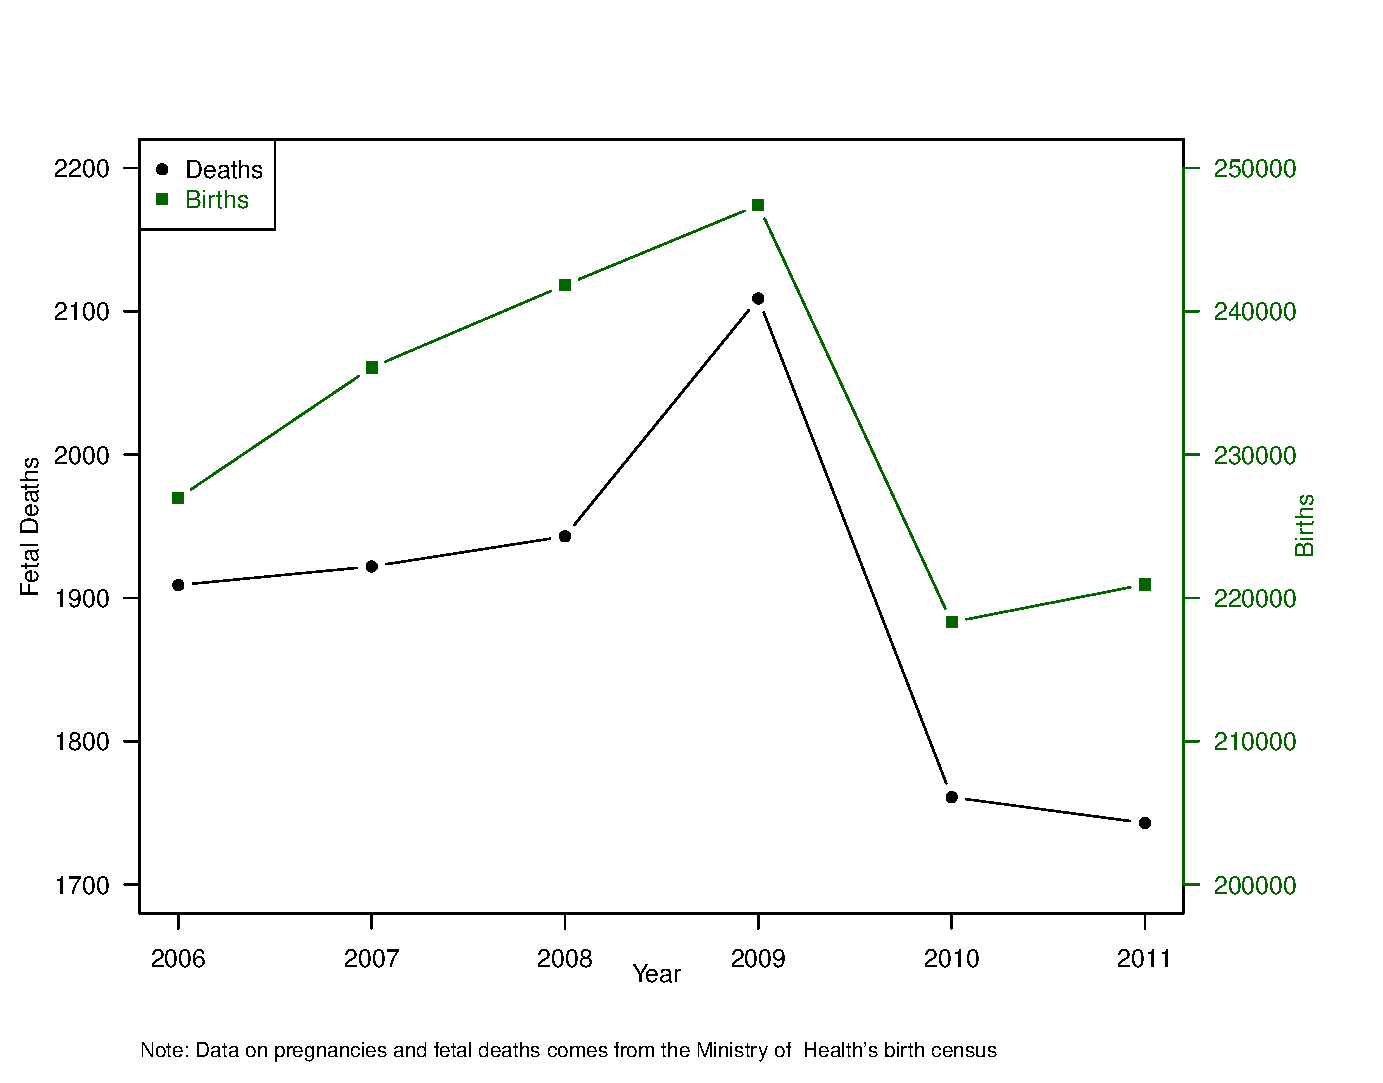
\includegraphics[scale=0.8, angle=90]{\teenfolder/Figures/BirthDeath.eps} 
%\end{center}
\end{figure}

\begin{figure}[htpb!]
\begin{center}
\caption{Pill Prescriptions and Availability by Time}
\vspace{-5mm}
\label{TEENfig:Pilltime}
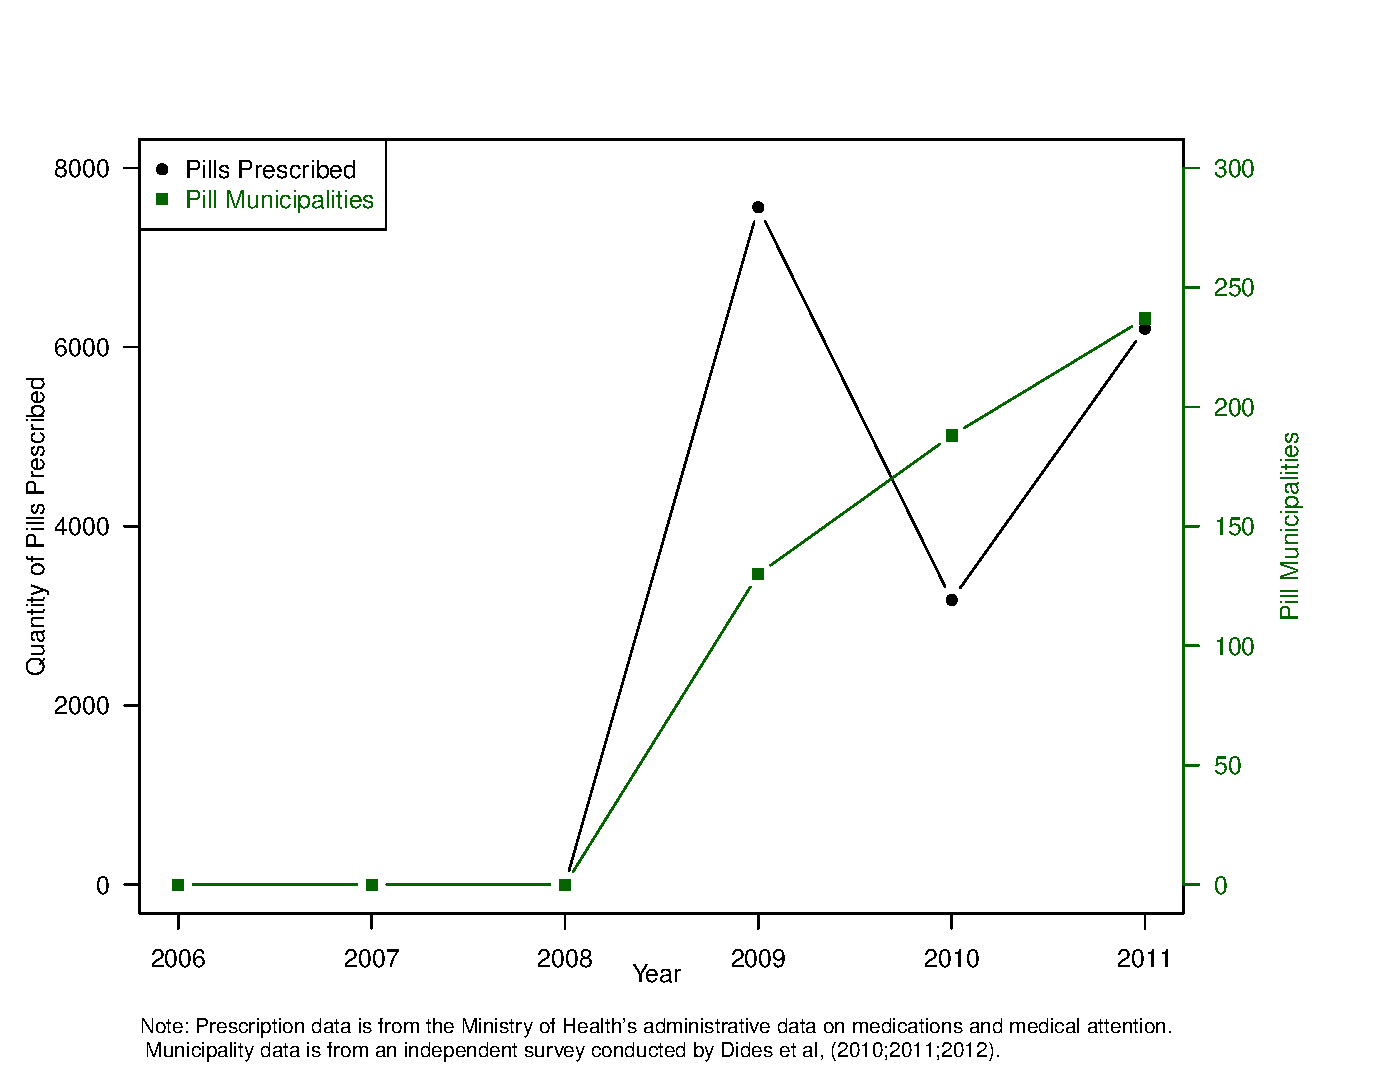
\includegraphics[scale=0.54]{\teenfolder/Figures/Pill.eps} 
\end{center}
\end{figure}

\begin{figure}[htpb!]
\begin{center}
\caption{Pregancies by Age Group and Time}
\vspace{-5mm}
\label{TEENfig:Pregtime}
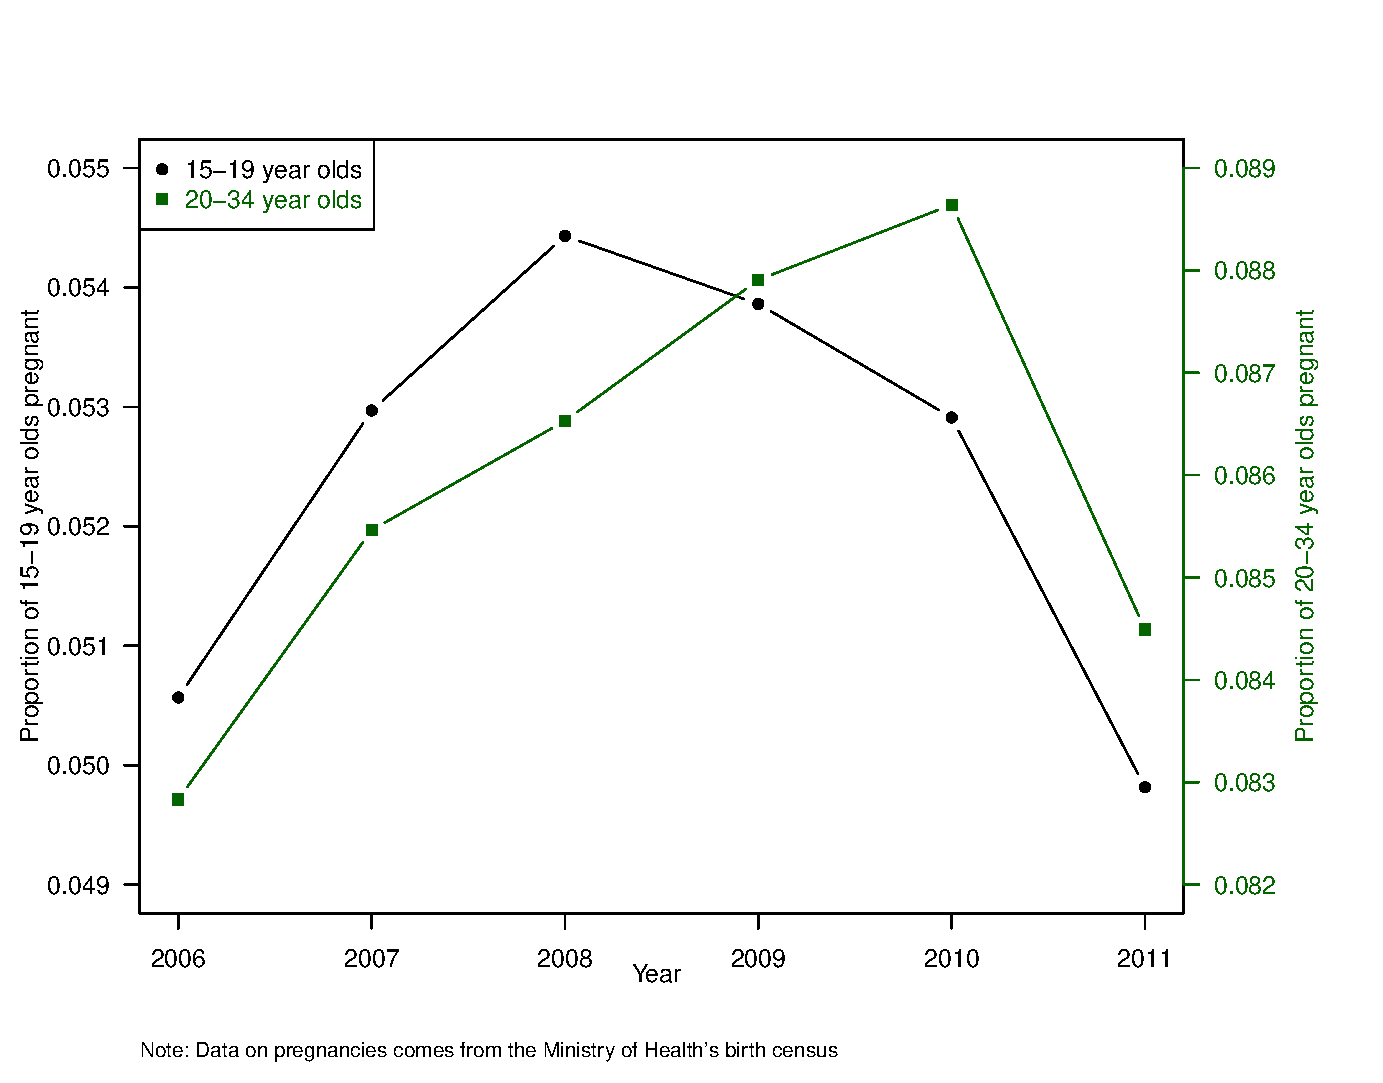
\includegraphics[scale=0.54]{\teenfolder/Figures/Births.eps} 
\end{center}
\end{figure}

\begin{figure}[htpb!]
\begin{center}
\caption{The Availability of the Pill by Geographic Region}
%NOTE: THIS FIGURES HAS BEEN REMOVED TO REDUCE FILE SIZE ON github
\label{TEENfig:PillGeo}
\includegraphics[scale=0.5]{\teenfolder/Results/Pill/Pill_l.eps} 
\end{center}
\end{figure}

\begin{figure}[htpb!]
\begin{center}
\caption{Estimates of $\hat\delta^c$ for Pregnancy (15-19)}
\label{TEENfig:Dist1519}
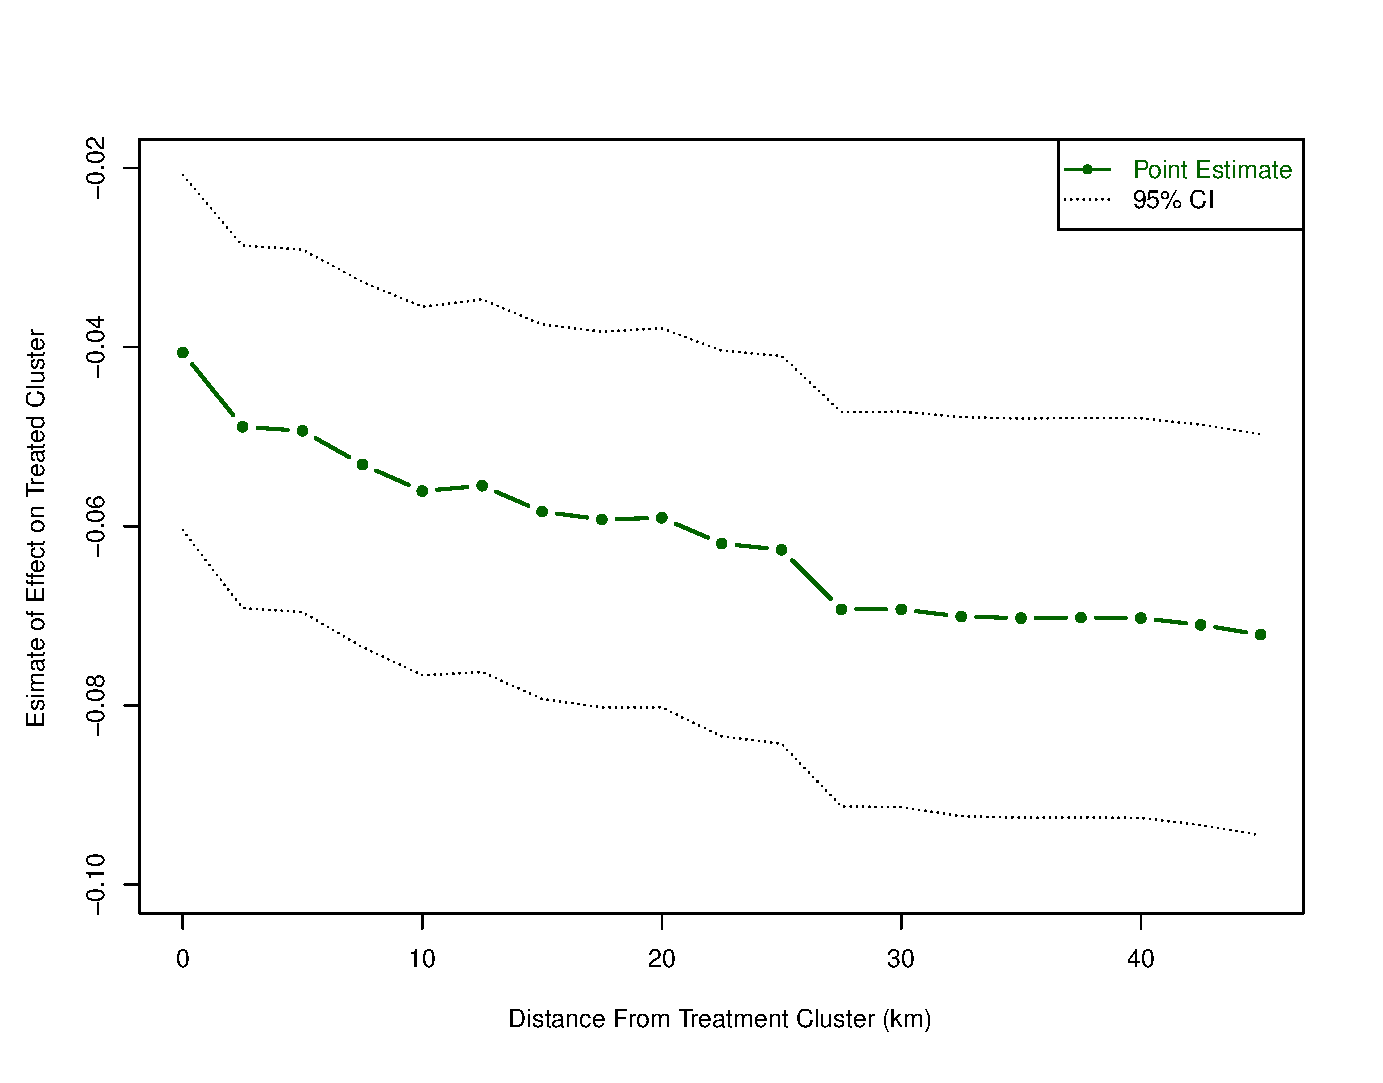
\includegraphics[scale=0.54]{\teenfolder/Figures/Dist1519.eps} 
\end{center}
\end{figure}

\begin{figure}[htpb!]
\begin{center}
\caption{Estimates of $\hat\delta^c$ for Pregnancy (20-34)}
\label{TEENfig:Dist2034}
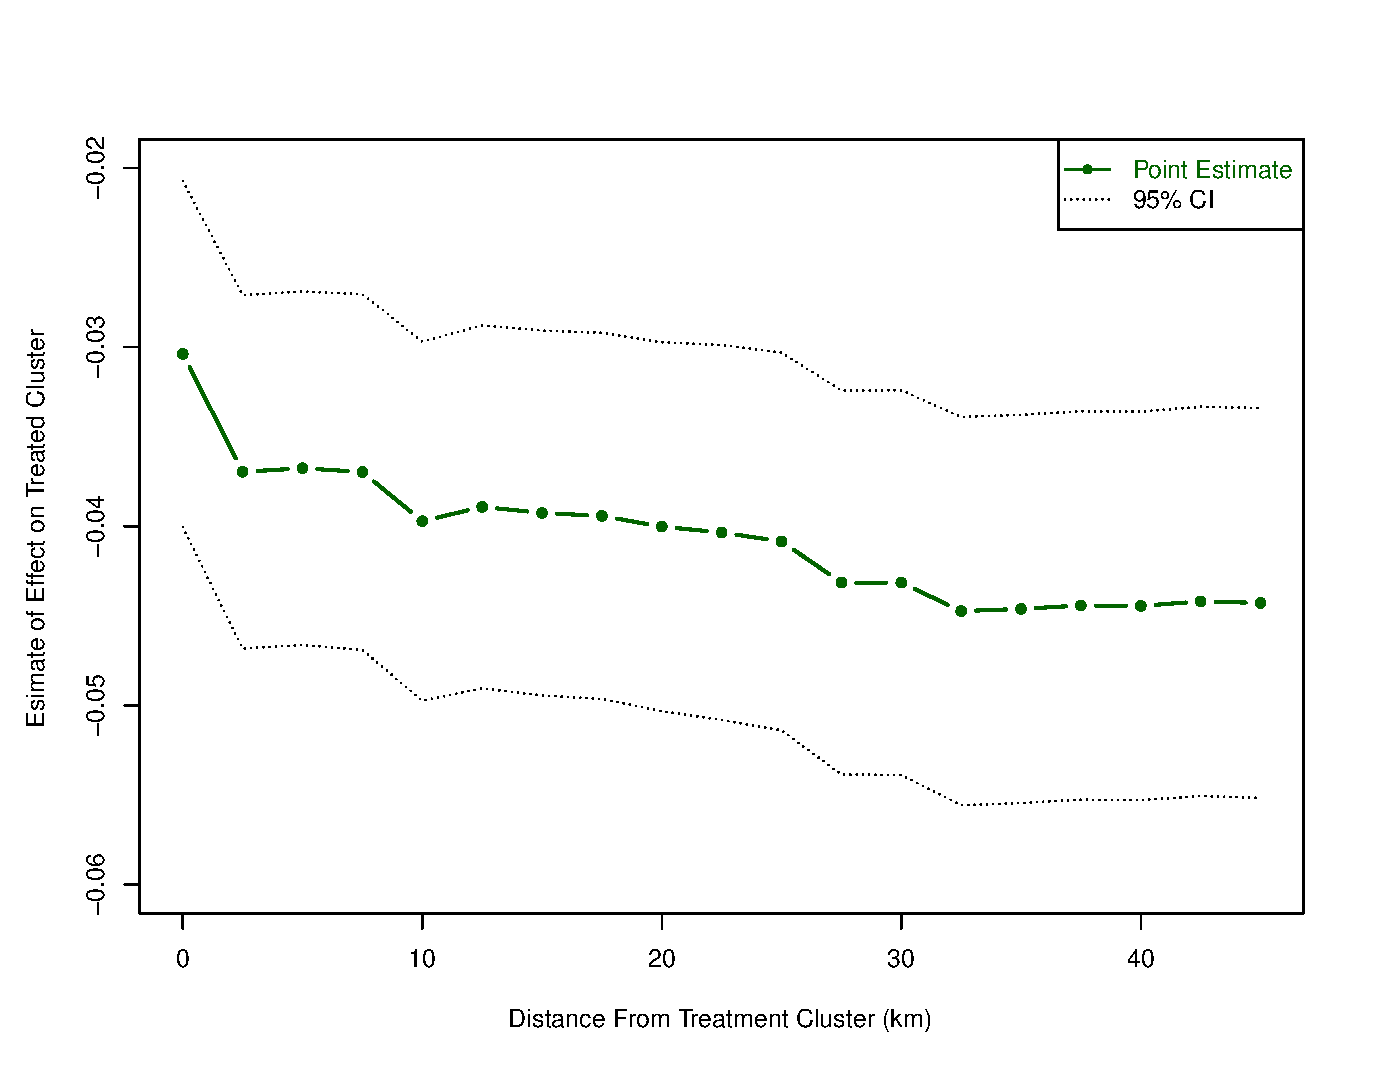
\includegraphics[scale=0.54]{\teenfolder/Figures/Dist2034.eps} 
\end{center}
\end{figure}

\begin{figure}[htpb!]
\begin{center}
\caption{Event Study: 15-19 Years}
\vspace{-5mm}
\label{TEENfig:Event1519}
\includegraphics[scale=0.54]{\teenfolder/Figures/Event1519.eps} 
\end{center}
\end{figure}

\begin{figure}[htpb!]
\begin{center}
\caption{Event Study: 20-34 Years}
\vspace{-5mm}
\label{TEENfig:Event2034}
\includegraphics[scale=0.54]{\teenfolder/Figures/Event2034.eps} 
\end{center}
\floatfoot{Note to figures \ref{TEENfig:Event1519}-\ref{TEENfig:Event2034}:
Points and confidence intervals represent estimates for a full event study.
Each point represents an indicator for the treatment group (pill municipality) 
interacted with $n$ years
prior or posterior to the reform.  On the $x$-axis, 0 represents the first year the 
reform arrived, 1 represents the reform having run for one year, and so forth.  
The (arbitrarily chosen) omitted base in each case is 3 years prior to the reform.}
\end{figure}

\clearpage

\section*{Tables}
\begin{table}[htpb!]
\caption{The Estimated Effect of Reforms on Fertility (Selected Studies)}
\label{TEENtab:lit}
\begin{tabular}{lcl} \toprule
Author & Effect (Std. Error) & Note \\ \midrule
\textbf{Panel A: The Contraceptive Pill} &&\\
\citet{Bailey2006}            & -0.074(0.057) & $a,(x=22)$  \\
\citet{Guldi2008}             & -0.085(0.041) &             \\
\citet{Bailey2009}            & 0.028(0.048)  & $a,(x=22)$  \\
\citet{KearnerLevine2009}     & -0.071(0.024) & $b$         \\
\citet{Bailey2012}            & -0.042(0.019) &             \\
\citet{OltmansHungerman2012}  & -0.088(0.023) &             \\
\textbf{Panel B: Abortion}&&\\
\citet{AngristEvans1996}      & -0.012(0.004) & $a,(x=19)$  \\
\citet{Levineetal1996}        & -0.019(0.007) & $c$         \\
\citet{Gruberetal1999}        & -0.059(0.005) & $d$         \\
\citet{Ananatetal2007}        & -0.068(0.012) & $a,(x=25)$  \\
\citet{Bailey2006}            & -0.093(0.043) & $a,(x=22)$  \\
\citet{Guldi2008}             & -0.100(0.054) &             \\
\citet{Bailey2009}            & -0.012(0.007) & $a,(x=22)$  \\
\citet{Ananatetal2009}        & -0.085(0.020) &             \\
\citet{OltmansHungerman2012}  & -0.043(0.015) &             \\
\citet{Valente2014}           & -0.073(0.027) & $e$         \\
\textbf{Panel C: The Morning After Pill}\\
\citet{Grossetal2014}         & -0.020(0.020) &             \\
\citet{Durrance2013}          & 0.006(0.036)  & $f$         \\
\bottomrule
\multicolumn{3}{p{11.2cm}}{\begin{footnotesize}\textsc{Note:} All figures 
report the results of short term access of a national fertility reform on 
birth rates of teenage (15-19 year old) women unless otherwise specified 
in notes. \newline 
$^a$ Binary model with outcome 1=first birth by age $x$. \newline
%\citet{Bailey2009} is an erratum for \citeyear{Bailey2006}.
$^b$ Estimate with no state trends reported.  With state trends: -0.047(0.013) \newline 
$^c$ Estimate expressed as births per woman.  Mean rate is 0.110 \newline 
$^d$ Estimate for states adopting 1974-1975. Estimate for 1971-1973 is 
-0.021(0.005). \newline
$^e$ This is the effect for all mothers.  When expressed as a rate, it is -8.1\% \newline
$^f$ State-specific analysis. Estimate is per additional \% of 
participating pharmacies
\end{footnotesize}} 
\end{tabular}
\end{table}




\begin{table}[htpb!] \centering
\caption{Summary Statistics} \label{TEENtab:SumStats}
\begin{tabular} {@{\extracolsep{5pt}}lp{3mm}ccc}\\ [-1.8ex]
\hline\hline\\ [-1.8ex] &&No Pill&Pill&Total \\
&&Available&Available& \\ \midrule 
\multicolumn{5}{l}{\textbf{Municipality Characteristics}} \\
&&&& \\
Poverty &&16.4&17.0&16.6\\
&&(7.47)&(7.56)&(7.49) \\
Conservative &&0.286&0.267&0.281\\
&&(0.452)&(0.443)&(0.45) \\
Education Spending (Total) &&4,817&5,980&5,108\\
&&(5,649)&(6,216)&(5,818) \\
Education Spending (Municipal) &&430,625&525,143&454,232\\
&&(873,448)&(858,240)&(870,635) \\
Health Spending &&1,866&2,788&2,096\\
&&(2,635)&(3,381)&(2,867) \\
Out of School &&4.07&3.98&4.05\\
&&(3.16)&(3.06)&(3.13) \\
Female Mayor &&0.120&0.134&0.123\\
&&(0.325)&(0.341)&(0.329) \\
Female Poverty &&60.5&62.0&60.8\\
&&(10.64)&(9.48)&(10.4) \\
Condom Use &&0.466&0.536&0.483\\
&&(0.0506)&(0.0401)&(0.0571) \\
Pill Distance &&204&0.00&153\\
&&(5,229)&(0.00)&(4,530) \\
\multicolumn{5}{l}{\textbf{Individual Characteristics}}\\
&&&& \\
Live Births &&0.054&0.053&0.054\\
&&(0.226)&(0.224)&(0.226) \\
Fetal Deaths &&0.0558&0.0513&0.0547\\
&&(0.269)&(0.256)&(0.266) \\
Birthweight &&3322.7&3334.3&3324.7\\
&&     (540.0)&     (542.3)&     (540.4)\\
Maternal education  &&       11.92&       12.03&       11.94\\
&&     (2.967)&     (2.894)&     (2.955)\\
Percent working     &&       0.295&       0.395&       0.312\\
&&     (0.456)&     (0.489)&     (0.463)\\
Married     &&       0.340&       0.309&       0.335\\
&&     (0.474)&     (0.462)&     (0.472)\\
Age at Birth      &&       27.05&       27.15&       27.07\\
&&     (6.777)&     (6.790)&     (6.779)\\ \midrule
N Comunas &&336&280&336\\
N Fetal Deaths &&9,999&3,064&13,063\\
N Births &&1,214,088&391,212&1,605,300\\
\hline \hline \\[-1.8ex]
\multicolumn{5}{p{12cm}}{\begin{footnotesize}\textsc{Notes:}
Group means are presented with standard deviations below in
parentheses.  Poverty refers to the \% of the municipality
below the poverty line, conservative is a binary variable
indicating if the mayor comes from a politically conservative
party (UDI or RN), health and education spending are measured
 in thousands of Chilean
pesos, and pill distance measures the distance (in km) to the
nearest municipality which reports prescribing emergency
contraceptives.  Pregnancies are reported as \% of all women
giving live birth, while fetal deaths are reported per live
birth.  All summary statistics are for the period 2006-2012.
\end{footnotesize}} \normalsize\end{tabular}\end{table}



\begin{table}
\caption{Comuna Characteristics and Pill Decisions}
\begin{center}
\begin{tabular}{l c c c c }
\toprule
 & EC Pill$\times$100 & EC Pill$\times$100 & Close$\times$100 & Close$\times$100 \\
&(1)&(2)&(3)&(4) \\ \midrule
Out of School       & $0.08$       & $0.06$       & $-0.05$     & $0.02$        \\
                    & $[0.15]$     & $[0.15]$     & $[0.14]$    & $[0.14]$      \\
Health Spending     & $-0.10$      & $-0.07$      & $-0.22$     & $-0.22$       \\
                    & $[0.19]$     & $[0.19]$     & $[0.17]$    & $[0.18]$      \\
Health Staff        & $0.16$       & $0.14$       & $0.40^{*}$  & $0.33$        \\
                    & $[0.26]$     & $[0.26]$     & $[0.24]$    & $[0.24]$      \\
Education Spending  & $-0.01$      & $-0.02$      & $-0.04^{*}$ & $-0.00$       \\
                    & $[0.02]$     & $[0.02]$     & $[0.02]$    & $[0.02]$      \\
Education Level     & $0.01$       & $0.04$       & $0.19^{*}$  & $0.06$        \\
                    & $[0.10]$     & $[0.11]$     & $[0.10]$    & $[0.11]$      \\
Female Poverty      & $0.12^{**}$  & $0.02$       & $0.00$      & $-0.02$       \\
                    & $[0.06]$     & $[0.07]$     & $[0.05]$    & $[0.06]$      \\
Female Workers      & $0.03$       & $0.02$       & $0.02$      & $-0.04$       \\
                    & $[0.07]$     & $[0.08]$     & $[0.07]$    & $[0.07]$      \\
Urban               & $-1.24$      & $-1.05$      & $2.14$      & $1.46$        \\
                    & $[1.45]$     & $[1.61]$     & $[1.35]$    & $[1.49]$      \\
Condom Use          & $17.73$      & $73.04^{**}$ & $11.52$     & $-56.97^{**}$ \\
                    & $[17.53]$    & $[29.79]$    & $[16.34]$   & $[27.57]$     \\
Condom Availability & $2.02$       & $16.55$      & $-16.96$    & $26.17$       \\
                    & $[15.58]$    & $[24.62]$    & $[14.52]$   & $[22.79]$     \\
Female Mayor        & $1.12$       & $2.18$       & $-1.85$     & $-1.29$       \\
                    & $[1.88]$     & $[1.90]$     & $[1.75]$    & $[1.76]$      \\
Conservative Mayor  & $-3.45^{**}$ & $-3.32^{**}$ & $2.11$      & $1.89$        \\
                    & $[1.40]$     & $[1.43]$     & $[1.31]$    & $[1.32]$      \\
Vote Margin         & $5.44$       & $5.89$       & $2.12$      & $4.70$        \\
                    & $[5.66]$     & $[5.81]$     & $[5.28]$    & $[5.38]$      \\
\midrule
R-squared           & 0.57         & 0.57         & 0.29        & 0.31          \\
Observations        & 2210         & 2210         & 2210        & 2210          \\
Year FE&Y&Y&Y&Y\\ Region FE &&Y&&Y\\ \bottomrule
\multicolumn{5}{p{12cm}}{\begin{footnotesize}\textsc{Notes:}
      Each column presents the results of an OLS regression of a municipality's treatment
      status (prescribes the EC pill, or close to a municipality which prescribes the
      EC pill), on municipal level characteristics.  Each outcome variable is binary,
      and has been multiplied by 100 for presentation.  Year fixed effects are
      always included.  Independent variables and their descriptive statistics
      are described in table \ref{TEENtab:SumStats} and the Data section of the paper.
      Standard errors clustered at the level of the municipality are displayed in
      parentheses. $^{*}$p$<$0.1; $^{**}$p$<$0.05; $^{***}$p$<$0.01\end{footnotesize}}
\end{tabular}
\label{TEENtab:pillchoice}
\end{center}
\end{table}


\begin{table}[!htbp] \centering
\caption{The Effect of the EC Pill on Birth Rates}
\label{TEENtab:aggregateASFR}
\begin{tabular}{@{\extracolsep{5pt}}lcccc}
\\[-1.8ex]\hline \hline \\[-1.8ex] 
& Birth& Birth& Birth& Birth\\
& Rate & Rate & Rate & Rate \\
&(1)&(2)&(3)&(4) \\ \hline
\multicolumn{5}{l}{\textbf{
\noindent Panel A: All Women}} \\
Emergency Contraceptive Pill     &$-$1.193$^{***}$&$-$2.247$^{***}$&$-$1.562$^{***}$&$-$1.721$^{***}$\\
            &[0.425]&[0.489]&[0.524]&[0.620]\\
 & & & & \\
Observations&2,210&2,210&2,210&2,210\\
Mean Birth Rate&53.87&53.87&53.87&53.87\\
 & & & & \\
\multicolumn{5}{l}{\noindent \textbf{
Panel B: 15-19 year olds}} \\
Emergency Contraceptive Pill&$-$3.811$^{***}$&$-$4.546$^{***}$&$-$2.795$^{**}$&$-$3.536$^{**}$\\
            &[0.714]&[1.179]&[1.218]&[1.538]\\
 & & & & \\
Observations&2,205&2,205&2,205&2,205\\
Mean Birth Rate&52.00&52.00&52.00&52.00\\
 & & & & \\
\multicolumn{5}{l}{\noindent \textbf{
Panel C: 20-34 year olds}} \\
Emergency Contraceptive Pill&$-$2.491$^{***}$&$-$3.277$^{***}$&$-$2.273$^{**}$&$-$2.452$^{**}$\\
            &[0.762]&[0.891]&[0.938]&[1.116]\\
 & & & & \\
Observations&2,210&2,210&2,210&2,210\\
Mean Birth Rate&85.49&85.49&85.49&85.49\\
 & & & & \\
\multicolumn{5}{l}{\noindent \textbf{
Panel B: 35-49 year olds}} \\
Emergency Contraceptive Pill&0.240&$-$0.586&$-$0.401&$-$0.106\\
            &[0.274]&[0.411]&[0.455]&[0.600]\\
 & & & & \\
Observations&2,210&2,210&2,210&2,210\\
Mean Birth Rate&21.40&21.40&21.40&21.40\\
\hline \\[-1.8ex] 
{\small Year \& Comuna FEs}             &Y&Y&Y&Y \\
{\small Municipal-Specific Linear Trends}& &Y&Y&Y \\
{\small Time Varying Controls}           & & &Y&Y \\
{\small Spillovers}                      & & & &Y \\
\hline \hline \\[-1.8ex]
\multicolumn{5}{p{12.8cm}}{\begin{footnotesize}
\textsc{Notes:} Each panel presents population-weighted
 difference-in-difference results for a regression of 
age-specific fertility rates (ASFR) on the EC reform for
 the age group in
 each municipality.  ASFR is defined as the number of   
births per 1,000 women.  In the case of all women, this 
is called the General Fertility Rate (GFR). All models  
are estimated by OLS, and each municipality is          
weighted by the population of women. Time varying       
controls included in the regression consist of party    
dummies for the mayor in power, the mayor's gender, the
 vote margin of the mayor, the percent of girls out of  
highschool, education spending spending by both the     
municipality and the Ministry of Education, total       
health spending and health spending on staff and        
training, the percent of female heads of households     
living below the poverty line, the percent of female    
workers in professional positions in the Municipality,  
and condom availability (measured at the level of the   
region). Standard errors are clustered at the level of  
the municipality.
$^{*}$p$<$0.1; $^{**}$p$<$0.05; $^{***}$p$<$0.01\end{footnotesize}}
\normalsize\end{tabular}\end{table}


\begin{landscape}
\begin{table}[!htbp] \centering
\caption{Alternative Specifications -- EC Pill and Births}
\label{TEENtab:BirthRobust}
\begin{tabular}{@{\extracolsep{5pt}}lcccccc}
\\[-1.8ex]\hline \hline \\[-1.8ex] 
&Double&Full    & No     &Inv & OLS   & OLS        \\
&Diff. &Controls& Weights&PS  & Count & ln(Birth)  \\ 
&(1)&(2)&(3)&(4)&(5)&(6) \\ \midrule
\multicolumn{7}{l}{\textbf{
\noindent Panel A: All Women}} \\
Emergency Contraceptive Pill & $-$1.193$^{***}$ & $-$1.721$^{***}$ & $-$1.789$^{***}$ & $-$1.167$^{*}$ & $-$25.936$^{***}$ & $-$0.029$^{**}$ \\
& [0.425] & [0.620] & [0.437] & [0.656] & [8.511] & [0.012] \\
 & & & & & & \\
Observations& 2,210 & 2,210 & 2,210 & 2,210 & 2,210 & 2,210 \\
Mean of Dep Var& 53.87 & 53.87 & 53.87 & 53.87 & 2632.67 & 7.37 \\
 & & & & & & \\ \multicolumn{7}{l}{\textbf{
\noindent Panel B: 15-19 year olds}} \\
Emergency Contraceptive Pill & $-$3.811$^{***}$ & $-$3.536$^{**}$ & $-$3.527$^{***}$ & $-$2.022 & $-$7.474$^{***}$ & $-$0.064$^{***}$ \\
& [0.714] & [1.538] & [0.700] & [1.999] & [2.275] & [0.024] \\
 & & & & & & \\
Observations& 2,205 & 2,205 & 2,205 & 2,205 & 2,205 & 2,205 \\
Mean of Dep Var& 52.00 & 52.00 & 52.00 & 52.00 & 386.14 & 5.46 \\
 & & & & & & \\ \multicolumn{7}{l}{\textbf{
\noindent Panel C: 20-34 year olds}} \\
Emergency Contraceptive Pill & $-$2.491$^{***}$ & $-$2.452$^{**}$ & $-$3.106$^{***}$ & $-$3.121$^{***}$ & $-$17.893$^{***}$ & $-$0.025$^{*}$ \\
& [0.762] & [1.116] & [0.810] & [0.927] & [6.101] & [0.014] \\
 & & & & & & \\
Observations& 2,210 & 2,210 & 2,210 & 2,210 & 2,210 & 2,210 \\
Mean of Dep Var& 85.49 & 85.49 & 85.49 & 85.49 & 1833.11 & 7.02 \\
 & & & & & & \\ \multicolumn{7}{l}{\textbf{
\noindent Panel D: 35-49 year olds}} \\
Emergency Contraceptive Pill & 0.240 & $-$0.106 & 0.099 & 0.388 & $-$0.541 & $-$0.010 \\
& [0.274] & [0.600] & [0.267] & [0.482] & [1.742] & [0.026] \\
 & & & & & & \\
Observations& 2,210 & 2,210 & 2,210 & 2,210 & 2,210 & 2,210 \\
Mean of Dep Var& 21.40 & 21.40 & 21.40 & 21.40 & 435.78 & 5.55 \\
\hline \\[-1.8ex] 
\multicolumn{7}{p{17.6cm}}{\begin{footnotesize}          
\textsc{Notes:}                                           
Column 1 replicates the diff-in-diff result from table     
\ref{TEENtab:aggregateASFR} column 1.  Column 2 estimates 
the same specification, however with full controls (our    
preferred specification).  Column 3 presents unweighted    
results of the preferred specification, and column 4       
weights using the inverse propensity score of the          
municipality's treatment status.  Columns 5 and 6 present 
results using alternative outcome measures.  These are the 
absolute number of births, and the log number of births    
plus 1 (respectively).  All standard errors are clustered  
at the level of the municipality. Full results with and    
without controls and trends for each specification are     
included in online appendix tables.                        
$^{*}$p$<$0.1; $^{**}$p$<$0.05; $^{***}$p$<$0.01\end{footnotesize}}
\normalsize\end{tabular}\end{table}\end{landscape}


\begin{table}[htpb!] \centering
\caption{The Effect of the EC Pill on Fetal Death Rates}
\label{TEENtab:DeathOLS}
\begin{tabular}{@{\extracolsep{5pt}}lccc}\\[-1.8ex]
\hline\hline\\[-1.8ex]
& All    & Early     & Late      \\
& Deaths & Gestation & Gestation \\ \midrule
\multicolumn{4}{l}{\noindent \textbf{
Panel A: All Women}} \\
Emergency Contraceptive Pill &0.313&$-$0.031&0.281\\
&[0.645]&[0.330]&[0.517]\\
& & & \\
Observations&2,189&2,189&2,189\\
Mean (fetal deaths/live birth)&8.14&2.40&4.76\\
&&&\\
\multicolumn{4}{l}{\noindent \textbf{
Panel B: 15-19 year olds}} \\
Emergency Contraceptive Pill &0.994&$-$1.344$^{*}$&2.175\\
&[1.674]&[0.730]&[1.467]\\
& & & \\
Observations&2,157&2,157&2,157\\
Mean (fetal deaths/live birth)&8.02&2.42&4.83\\
&&&\\
\multicolumn{4}{l}{\noindent \textbf{
Panel C: 20-34 year olds}} \\
Emergency Contraceptive Pill &0.378&0.394&0.071\\
&[0.691]&[0.350]&[0.630]\\
& & & \\
Observations&2,184&2,184&2,184\\
Mean (fetal deaths/live birth)&7.37&2.21&4.35\\
&&&\\
\multicolumn{4}{l}{\noindent \textbf{
Panel C: 35-49 year olds}} \\
Emergency Contraceptive Pill &$-$0.540&$-$0.227&$-$0.512\\
&[2.032]&[1.512]&[1.400]\\
& & & \\
Observations&2,159&2,159&2,153\\
Mean (fetal deaths/live birth)&11.47&3.21&6.23\\
\hline \hline \\[-1.8ex]
\multicolumn{4}{p{10.2cm}}{\begin{footnotesize}          
\textsc{Notes:} Each panel presents weighted difference-
in-difference results for a regression of the fetal      
death rate (deaths per 1,000 live births) on the EC      
reform for the age group in question. All models are     
estimated by OLS, and each municipality is weighted by   
the number of live births. All regressions include the   
controls documented in table \ref{TEENtab:aggregateASFR}.
Standard errors are clustered at the level of the        
municipality.
$^{*}$p$<$0.1; $^{**}$p$<$0.05; $^{***}$p$<$0.01;\end{footnotesize}}
\normalsize\end{tabular}\end{table}


\begin{landscape}\begin{table}[htpb!]\centering
\caption{Emergency Contraception and Aggregate Human Capital} \label{TEENtab:PillAgg}
\begin{tabular}{@{\extracolsep{5pt}}lccccccccc} \\
[-1.8ex]\hline\hline \\[-1.8ex] &\multicolumn{3}{c}{15-19 year olds} &\multicolumn{3}{c}{20-34 year olds} &\multicolumn{3}{c}{35-49 year olds} \\
\cmidrule(r){2-4} \cmidrule(r){5-7} \cmidrule(r){8-10}
\textsc{Panel A:}&(1)&(2)&(3)&(4)&(5)&(6)&(7)&(8)&(9) \\
\textsc{Mother Characteristics} & Yrs Educ & Working & Married& Yrs Educ & Working & Married & Yrs Educ & Working & Married\\ \midrule
 & & & & & & & & & \\
Morning After Pill & 0.022 & -0.002 & 0.000& 0.001 & -0.004* & -0.003& 0.061** & -0.004 & -0.001 \\
& (0.021) & (0.002) & (0.001)& (0.014) & (0.002) & (0.005)& (0.028) & (0.005) & (0.007) \\
 & & & & & & & & & \\
Observations & 131,605 & 131,746 & 131,614& 896,230 & 897,363 & 896,318& 198,885 & 199,472 & 198,906\\
$ R^2 $ &  0.02 & 0.01 & 0.01& 0.14 & 0.04 & 0.17& 0.21 & 0.03 & 0.247 \\
 & & & & & & & & & \\
 & & & & & & & & & \\ \midrule
\textsc{Panel B:}&(1)&(2)&(3)&(4)&(5)&(6)&(7)&(8)&(9) \\
\textsc{Child Characteristics} & Weight & Gestation & Length& Weight & Gestation & Length & Weight & Gestation & Length\\ \midrule
 & & & & & & & & & \\
Morning After Pill & -1.377 & -0.020 & 0.039& -0.636 & -0.023*** & 0.02& -4.923 & -0.016 & 0.030 \\
& (5.944) & (0.019) & (0.028)& (2.532) & (0.008) & (0.016)& (5.602) & (0.016) & (0.024) \\
 & & & & & & & & & \\
Observations & 131,746 & 131,471 & 129,880& 897,363 & 895,671 & 885,932& 199,472 & 198,745 & 195,863\\
$ R^2 $ & 0.01 & 0.01 & 0.03& 0.01 & 0.01 & 0.03& 0.09 & 0.01 & 0.03 \\ \hline \hline \\[-1.8ex]
\multicolumn{10}{p{21cm}}{\begin{footnotesize}\textsc{Notes:} Each column represents an OLS regression, and full controls listed in table
\ref{TEENtab:PillPreg} are included.  Working and Married are binary variables, Weight is measured in grams, Gestation in weeks, and Length
in centimetres.  Summary statistics for these variables are available in table \ref{TEENtab:SumStats}.  Standard errors are clustered at the
 level of the municipality. $^{*}$ p $<0.1$; $^{**}$ p $<0.05$; $^{***}$ p $<0.01$.\end{footnotesize}}
\normalsize\end{tabular}\end{table}\end{landscape}


\begin{table}[!htbp] \centering
\caption{The Morning After Pill and Treatment Spillovers}
\label{TEENtab:Spillover} 
\scalebox{0.5}{\begin{tabular}
{@{\extracolsep{5pt}}lccc}\\[-1.8ex]\hline\hline\\
[-1.8ex] & 15-19 & 20-34 & 35-49 \\
& Year olds & Year olds & Year olds \\ \midrule
\multicolumn{4}{l}{\textsc{\noindent Panel A: Births}} \\
& & & \\
Morning After Pill &$-$0.091$^{***}$&$-$0.053$^{***}$&0.016\\
&(0.016)&(0.013)&(0.014)\\
Close $<15$ km &$-$0.083$^{***}$&$-$0.044$^{***}$&0.019\\
&(0.021)&(0.014)&(0.016)\\
Close 15-30 km &$-$0.078$^{***}$&$-$0.024$^{*}$& \\
&(0.022)&(0.013)& \\
Close 30-45 km &$-$0.057&$-$0.026& \\
&(0.036)&(0.031)& \\
& & & \\
Observations&4,152,490&11,022,111&10,572,196\\
McFadden's $R^2$&0.673&0.774&0.538\\ \midrule
\multicolumn{4}{l}{\textsc{\noindent Panel B: Fetal Deaths}}\\
&&&\\
Morning After Pill &$-$0.935$^{***}$&$-$0.230$^{*}$&$-$0.785$^{***}$\\
&(0.217)&(0.125)&(0.230)\\
Close $<15$ km &$-$0.163&$-$0.031& 0.051\\
&(0.234)&(0.151)&(0.226)\\
&&&\\
Observations&218,388&949,477&227,029\\
McFadden's $R^2$&0.379&0.386&0.412\\
\hline \hline \\[-1.8ex]
\end{tabular}}\end{table}


\newpage

\biblioinc

%\section{Appendix Tables}
%\begin{table}[!htbp] \centering
\caption{The Effect of the EC Pill on Total Births}
\label{TEENtab:aggregate}
\begin{tabular}{@{\extracolsep{5pt}}lcccc}
\\[-1.8ex]\hline \hline \\[-1.8ex] 
& Number& Number & Number & Number \\
& Births& Births & Births & Births \\
&(1)&(2)&(3)&(4) \\ \hline
\multicolumn{5}{l}{\textbf{
\noindent Panel A: All Women}} \\
Emergency Contraceptive Pill&7.623&$-$27.564$^{***}$&$-$20.337$^{***}$&$-$25.936$^{***}$\\
            &[5.720]&[5.242]&[5.954]&[8.511]\\
 & & & & \\
Observations&2,210&2,210&2,210&2,210\\
Mean Number of Births&2632.67&2632.67&2632.67&2632.67\\
 & & & & \\
\multicolumn{5}{l}{\noindent \textbf{
Panel B: 15-19 year olds}} \\
Emergency Contraceptive Pill&$-$8.618$^{***}$&$-$8.519$^{***}$&$-$5.583$^{***}$&$-$7.474$^{***}$\\
            &[1.233]&[1.517]&[1.716]&[2.275]\\
 & & & & \\
Observations&2,205&2,205&2,205&2,205\\
Mean Number of Births&386.14&386.14&386.14&386.14\\
 & & & & \\
\multicolumn{5}{l}{\noindent \textbf{
Panel C: 20-34 year olds}} \\
Emergency Contraceptive Pill&11.605$^{***}$&$-$16.644$^{***}$&$-$12.890$^{***}$&$-$17.893$^{***}$\\
            &[4.173]&[3.621]&[4.257]&[6.101]\\
 & & & & \\
Observations&2,210&2,210&2,210&2,210\\
Mean Number of Births&1833.11&1833.11&1833.11&1833.11\\
 & & & & \\
\multicolumn{5}{l}{\noindent \textbf{
Panel B: 35-49 year olds}} \\
Emergency Contraceptive Pill&4.636$^{***}$&$-$2.401$^{*}$&$-$1.843&$-$0.541\\
            &[1.608]&[1.299]&[1.371]&[1.742]\\
 & & & & \\
Observations&2,210&2,210&2,210&2,210\\
Mean Number of Births&435.78&435.78&435.78&435.78\\
\hline \\[-1.8ex] 
{\small Year \& Comuna FEs}             &Y&Y&Y&Y \\
{\small Municipal-Specific Linear Trends}& &Y&Y&Y \\
{\small Time Varying Controls}           & & &Y&Y \\
{\small Spillovers}                      & & & &Y \\
\hline \hline \\[-1.8ex]
\multicolumn{5}{p{14.2cm}}{\begin{footnotesize}
\textsc{Notes:} Each panel presents population       
weighted difference-in-difference results for a       
regression of the total number of births for the age  
group in each municipality. Specifications are        
identical to table \ref{TEENtab:aggregateASFR},      
however birth weights are replaced by the total number
 of births. Standard errors are clustered             
at the level of the municipality.
$^{*}$p$<$0.1; $^{**}$p$<$0.05; $^{***}$p$<$0.01\end{footnotesize}}
\normalsize\end{tabular}\end{table}

\begin{table}[!htbp] \centering
\caption{The Effect of the EC Pill on Birth Rates}
\label{TEENtab:aggregateASFR}
\begin{tabular}{@{\extracolsep{5pt}}lcccc}
\\[-1.8ex]\hline \hline \\[-1.8ex] 
& Birth& Birth& Birth& Birth\\
& Rate & Rate & Rate & Rate \\
&(1)&(2)&(3)&(4) \\ \hline
\multicolumn{5}{l}{\textbf{
\noindent Panel A: All Women}} \\
Emergency Contraceptive Pill     &$-$1.193$^{***}$&$-$2.247$^{***}$&$-$1.562$^{***}$&$-$1.721$^{***}$\\
            &[0.425]&[0.489]&[0.524]&[0.620]\\
 & & & & \\
Observations&2,210&2,210&2,210&2,210\\
Mean Birth Rate&53.87&53.87&53.87&53.87\\
 & & & & \\
\multicolumn{5}{l}{\noindent \textbf{
Panel B: 15-19 year olds}} \\
Emergency Contraceptive Pill&$-$3.811$^{***}$&$-$4.546$^{***}$&$-$2.795$^{**}$&$-$3.536$^{**}$\\
            &[0.714]&[1.179]&[1.218]&[1.538]\\
 & & & & \\
Observations&2,205&2,205&2,205&2,205\\
Mean Birth Rate&52.00&52.00&52.00&52.00\\
 & & & & \\
\multicolumn{5}{l}{\noindent \textbf{
Panel C: 20-34 year olds}} \\
Emergency Contraceptive Pill&$-$2.491$^{***}$&$-$3.277$^{***}$&$-$2.273$^{**}$&$-$2.452$^{**}$\\
            &[0.762]&[0.891]&[0.938]&[1.116]\\
 & & & & \\
Observations&2,210&2,210&2,210&2,210\\
Mean Birth Rate&85.49&85.49&85.49&85.49\\
 & & & & \\
\multicolumn{5}{l}{\noindent \textbf{
Panel B: 35-49 year olds}} \\
Emergency Contraceptive Pill&0.240&$-$0.586&$-$0.401&$-$0.106\\
            &[0.274]&[0.411]&[0.455]&[0.600]\\
 & & & & \\
Observations&2,210&2,210&2,210&2,210\\
Mean Birth Rate&21.40&21.40&21.40&21.40\\
\hline \\[-1.8ex] 
{\small Year \& Comuna FEs}             &Y&Y&Y&Y \\
{\small Municipal-Specific Linear Trends}& &Y&Y&Y \\
{\small Time Varying Controls}           & & &Y&Y \\
{\small Spillovers}                      & & & &Y \\
\hline \hline \\[-1.8ex]
\multicolumn{5}{p{12.8cm}}{\begin{footnotesize}
\textsc{Notes:} Each panel presents population-weighted
 difference-in-difference results for a regression of 
age-specific fertility rates (ASFR) on the EC reform for
 the age group in
 each municipality.  ASFR is defined as the number of   
births per 1,000 women.  In the case of all women, this 
is called the General Fertility Rate (GFR). All models  
are estimated by OLS, and each municipality is          
weighted by the population of women. Time varying       
controls included in the regression consist of party    
dummies for the mayor in power, the mayor's gender, the
 vote margin of the mayor, the percent of girls out of  
highschool, education spending spending by both the     
municipality and the Ministry of Education, total       
health spending and health spending on staff and        
training, the percent of female heads of households     
living below the poverty line, the percent of female    
workers in professional positions in the Municipality,  
and condom availability (measured at the level of the   
region). Standard errors are clustered at the level of  
the municipality.
$^{*}$p$<$0.1; $^{**}$p$<$0.05; $^{***}$p$<$0.01\end{footnotesize}}
\normalsize\end{tabular}\end{table}


%\begin{table}[htpb!] \centering 
  \caption{The Morning After Pill and Pregnancy: Full Covariates} 
  \label{TEENtabPregFull} 
\begin{tabular}{@{\extracolsep{5pt}}lccc} 
\\[-1.8ex]\hline 
\hline \\[-1.8ex] 
 & \multicolumn{3}{c}{Pregnancy} \\ 
\cline{2-4} 
\\[-1.8ex] & 15-19 & 20-34 & 35-49 \\ 
 & year olds & year olds & year olds \\ 
\\[-1.8ex] & \multicolumn{1}{c}{(1)} & \multicolumn{1}{c}{(2)} & \multicolumn{1}{c}{(3)}\\ 
\hline \\[-1.8ex] 

 Morning After Pill & -0.041$^{***}$ & -0.030$^{***}$ & 0.006 \\ 
  & (0.010) & (0.005) & (0.010) \\ 
  & & & \\ 
 Female Mayor & 0.016 & -0.005 & -0.007 \\ 
  & (0.026) & (0.013) & (0.026) \\ 
  & & & \\ 
 Mayor's Support & 0.054 & 0.017 & -0.129 \\ 
  & (0.084) & (0.042) & (0.085) \\ 
  & & & \\ 
 Out of School & -0.004 & -0.001 & -0.001 \\ 
  & (0.003) & (0.001) & (0.003) \\ 
  & & & \\ 
 Total Education Spending & 0.001$^{*}$ & -0.00004 & 0.001$^{**}$ \\ 
  & (0.0003) & (0.0002) & (0.0003) \\ 
  & & & \\ 
 Municipal Education Spending & -0.004$^{***}$ & -0.001$^{**}$ & -0.001$^{**}$ \\ 
  & (0.001) & (0.0003) & (0.001) \\ 
  & & & \\ 
 Health Spending & -0.0002 & 0.0001 & -0.0005 \\ 
  & (0.001) & (0.0003) & (0.001) \\ 
  & & & \\ 
 Health Training & -0.080$^{***}$ & -0.036$^{***}$ & 0.005 \\ 
  & (0.024) & (0.012) & (0.025) \\ 
  & & & \\ 
 Health Staff & 0.001 & 0.001$^{***}$ & -0.0004 \\ 
  & (0.001) & (0.0005) & (0.001) \\ 
  & & & \\ 
 Female Poverty & -0.0004 & -0.0001 & 0.002$^{***}$ \\ 
  & (0.001) & (0.0003) & (0.001) \\ 
  & & & \\ 
 Female Workers & -0.001 & -0.0005 & 0.001 \\ 
  & (0.001) & (0.0004) & (0.001) \\ 
  & & & \\ 
\hline \\[-1.8ex] 
Years $\times$ Municipality & 1,929 & 1,934 & 1,934 \\ 
\hline 
\hline \\[-1.8ex] 
\multicolumn{4}{p{10.8cm}}{\begin{footnotesize} \textsc{Notes:} Each model is identical to 
            column (4) of table \ref{TEENtab:PillPreg}.  A description of each 
            variable is also provided in table \ref{TEENtab:PillPreg}.  Municipality
            dummies and trends and political party dummies have been omitted for 
            clarity. $^{*}$p$<$0.1; $^{**}$p$<$0.05; $^{***}$p$<$0.01 
            \end{footnotesize}} \\ 
\end{tabular} 
\end{table} 


%\begin{table}[htpb!] \centering 
  \caption{The Morning After Pill and Fetal Death: Full Covariates} 
  \label{TEENtabDeathFull} 
\begin{tabular}{@{\extracolsep{5pt}}lccc} 
\\[-1.8ex]\hline 
\hline \\[-1.8ex] 
 & \multicolumn{3}{c}{Fetal Death (0-20 Weeks)} \\ 
\cline{2-4} 
\\[-1.8ex] & 15-19 & 20-34 & 35-49 \\ 
 & year olds & year olds & year olds \\ 
\\[-1.8ex] & \multicolumn{1}{c}{(1)} & \multicolumn{1}{c}{(2)} & \multicolumn{1}{c}{(3)}\\ 
\hline \\[-1.8ex] 
 Morning After Pill & -0.815$^{***}$ & -0.189$^{*}$ & -0.776$^{***}$ \\ 
  & (0.237) & (0.113) & (0.217) \\ 
  & & & \\ 
  Female Mayor & 0.987$^{*}$ & 0.096 & -0.270 \\ 
  & (0.593) & (0.293) & (0.528) \\ 
  & & & \\ 
  Mayor's Support & 1.861 & 1.168 & -0.416 \\ 
  & (1.886) & (0.989) & (1.783) \\ 
  & & & \\ 
  Out of School & -0.005 & -0.003 & 0.074 \\ 
  & (0.083) & (0.032) & (0.064) \\ 
  & & & \\ 
  Total Education Spending & 0.0001 & -0.00003 & -0.00003 \\ 
  & (0.0001) & (0.00004) & (0.0001) \\ 
  & & & \\ 
  Municipal Education Spending & 0.0004$^{*}$ & 0.0001 & 0.0001 \\ 
  & (0.0002) & (0.0001) & (0.0001) \\ 
  & & & \\ 
  Health Spending & -0.0001 & 0.0002$^{**}$ & 0.0001 \\ 
  & (0.0002) & (0.0001) & (0.0001) \\ 
  & & & \\ 
  Health Training & 0.005 & -0.003 & 0.005 \\ 
  & (0.004) & (0.002) & (0.004) \\ 
  & & & \\ 
  Health Staff & 0.00004 & 0.00004 & 0.0001 \\ 
  & (0.0002) & (0.0001) & (0.0002) \\ 
  & & & \\ 
  Female Poverty & 0.017 & 0.002 & 0.002 \\ 
  & (0.016) & (0.007) & (0.013) \\ 
  & & & \\ 
  Female Workers & 0.008 & -0.006 & 0.018 \\ 
  & (0.019) & (0.008) & (0.014) \\ 
  & & & \\ 
 \hline \\[-1.8ex] 
Years $\times$ Municipality & \multicolumn{1}{c}{1,887} & \multicolumn{1}{c}{1,912} & \multicolumn{1}{c}{1,891} \\ 
Akaike Inf. Crit. & \multicolumn{1}{c}{2,594.943} & \multicolumn{1}{c}{4,244.940} & \multicolumn{1}{c}{2,811.065} \\ 
\hline 
\hline \\[-1.8ex] 
\multicolumn{4}{p{10.8cm}}{\begin{footnotesize} \textsc{Notes:} Each model is identical to 
          column (2) of table \ref{TEENtab:PillDeath}.  A description of each 
          variable is also provided in table \ref{TEENtab:PillPreg}.  Municipality
          dummies and trends and political party dummies have been omitted for 
          clarity. $^{*}$p$<$0.1; $^{**}$p$<$0.05; $^{***}$p$<$0.01 
          \end{footnotesize}} \\ 
\normalsize 
\end{tabular} 
\end{table} 



\begin{table}[!htbp] \centering
\caption{Back of the Envelope Calculation of Effect Sizes}
\label{TEENtab:BOE}
\scalebox{0.7}{
\begin{tabular}{@{\extracolsep{5pt}}lcc}
\\[-1.8ex]\hline \hline \\[-1.8ex] 
& 18 \& Under & 19 \& Over\\ 
&(1)&(2) \\ \hline
 & &  \\
Morning After Pill &$-$0.069$^{***}$&$-$0.032$^{***}$\\
&(0.019)&(0.010)\\
Close $<15$ km &$-$0.075$^{***}$&$-$0.032$^{***}$\\
&(0.026)&(0.012)\\
Close 15-30 km &$-$0.049$^{*}$&$-$0.013\\
&(0.028)&(0.012)\\
& & \\ \midrule
N Preg (pill) &20,713&172,557\\
N Preg (close 15) &10,370&100,749\\
N Preg (close 30) &6,141&48,756\\
Pills Disbursed & 5,736 & 11,121 \\
\hline \hline \\[-1.8ex]
\multicolumn{3}{p{7.2cm}}{\begin{footnotesize}\textsc{Notes:} 
$^{*}$p$<$0.1; $^{**}$p$<$0.05; $^{***}$p$<$0.01\end{footnotesize}}
\normalsize\end{tabular}}\end{table}







%\appendix
%\section*{Online Appendix}
%\section{Data Agreement with Government of Chile}
%\includepdf[pages={-}]{\teenfolder/Data/DECLARACION_CONFIDENCIALIDAD.pdf}
